\documentclass[10pt,journal,compsoc]{IEEEtran}

% === CRITICAL: ToUnicode mapping for correct text extraction ===
% cmap must be loaded BEFORE font packages to ensure proper character mapping
\usepackage{cmap}
% Enable glyph-to-unicode mapping (improves PDF text extraction fidelity)
\input{glyphtounicode}
\pdfgentounicode=1

\ifCLASSOPTIONcompsoc
  \usepackage[nocompress]{cite}
\else
  \usepackage{cite}
\fi
% Override Palatino with Times (required for IEEE TDSC)
\usepackage{mathptmx}
\usepackage{fix-cm}
\usepackage{amsmath,amssymb}
\usepackage{graphicx}
\usepackage{array}
\usepackage{booktabs}
\usepackage{url}
\usepackage{xurl}
\urlstyle{same}
\Urlmuskip=0mu
% Reset xurl's default lowercase breaks and use controlled break points only
\makeatletter
% Clear any lowercase letter break points that xurl may have added
% Note: Removed hyphen from UrlBreaks to prevent soft-hyphen artifacts (U+00AD) in extracted text
\def\UrlBreaks{\do\.\do\@\do\/\do\\\do\!\do\_\do\|\do\;\do\>\do\]\do\)\do\,\do\?\do\'\do\+\do\=\do\#}
% Prefer breaking at path separators and colons
\def\UrlBigBreaks{\do\/\do\:}
% Do NOT add \UrlOrds or lowercase letters
\makeatother
\usepackage[T1]{fontenc}  % Better font encoding for text extraction
\usepackage[tracking=false,letterspace=0]{microtype}  % Disable letterspace to prevent char spreading
\microtypesetup{expansion=false}  % Disable font expansion for tt fonts
\usepackage[hidelinks]{hyperref}
% PDF Metadata for indexing and compliance
\hypersetup{
    pdftitle={},
    pdfauthor={},
    pdfkeywords={},
    pdfsubject={}
}
\hbadness=10000
\vbadness=10000
\usepackage{xr}
% Allow main paper to reference Supplementary Table/Figure numbers via \ref{}.
% Build TDSC supplementary once so TDSC supplementary .aux exists.
\makeatletter
\IfFileExists{TDSC-2026-01-0318_supplementary.aux}{\externaldocument{TDSC-2026-01-0318_supplementary}}{}
\makeatother
\usepackage{xcolor}
\usepackage{fvextra}
\fvset{breaklines=true,breakanywhere=true,breakautoindent=false,breakindent=0pt,fontsize=\small}
\newcommand{\VerbBar}{|}
\newcommand{\VERB}{\Verb[commandchars=\\\{\}]}
\DefineVerbatimEnvironment{Highlighting}{Verbatim}{commandchars=\\\{\},breaklines=true,breakanywhere=true,breakautoindent=false,breakindent=0pt,fontsize=\small}
\newenvironment{Shaded}{}{}
\newcommand{\AlertTok}[1]{\textcolor[rgb]{1.00,0.00,0.00}{\textbf{#1}}}
\newcommand{\AnnotationTok}[1]{\textcolor[rgb]{0.38,0.63,0.69}{\textbf{\textit{#1}}}}
\newcommand{\AttributeTok}[1]{\textcolor[rgb]{0.49,0.56,0.16}{#1}}
\newcommand{\BaseNTok}[1]{\textcolor[rgb]{0.25,0.63,0.44}{#1}}
\newcommand{\BuiltInTok}[1]{\textcolor[rgb]{0.00,0.50,0.00}{\textbf{#1}}}
\newcommand{\CharTok}[1]{\textcolor[rgb]{0.25,0.44,0.63}{#1}}
\newcommand{\CommentTok}[1]{\textcolor[rgb]{0.38,0.63,0.69}{\textit{#1}}}
\newcommand{\CommentVarTok}[1]{\textcolor[rgb]{0.38,0.63,0.69}{\textbf{\textit{#1}}}}
\newcommand{\ConstantTok}[1]{\textcolor[rgb]{0.53,0.00,0.00}{#1}}
\newcommand{\ControlFlowTok}[1]{\textcolor[rgb]{0.00,0.44,0.13}{\textbf{#1}}}
\newcommand{\DataTypeTok}[1]{\textcolor[rgb]{0.56,0.13,0.00}{#1}}
\newcommand{\DecValTok}[1]{\textcolor[rgb]{0.25,0.63,0.44}{#1}}
\newcommand{\DocumentationTok}[1]{\textcolor[rgb]{0.73,0.13,0.13}{\textit{#1}}}
\newcommand{\ErrorTok}[1]{\textcolor[rgb]{1.00,0.00,0.00}{\textbf{#1}}}
\newcommand{\ExtensionTok}[1]{#1}
\newcommand{\FloatTok}[1]{\textcolor[rgb]{0.25,0.63,0.44}{#1}}
\newcommand{\FunctionTok}[1]{\textcolor[rgb]{0.02,0.16,0.49}{#1}}
\newcommand{\ImportTok}[1]{\textcolor[rgb]{0.00,0.50,0.00}{\textbf{#1}}}
\newcommand{\InformationTok}[1]{\textcolor[rgb]{0.38,0.63,0.69}{\textbf{\textit{#1}}}}
\newcommand{\KeywordTok}[1]{\textcolor[rgb]{0.00,0.44,0.13}{\textbf{#1}}}
\newcommand{\NormalTok}[1]{#1}
\newcommand{\OperatorTok}[1]{\textcolor[rgb]{0.40,0.40,0.40}{#1}}
\newcommand{\OtherTok}[1]{\textcolor[rgb]{0.00,0.44,0.13}{#1}}
\newcommand{\PreprocessorTok}[1]{\textcolor[rgb]{0.74,0.48,0.00}{#1}}
\newcommand{\RegionMarkerTok}[1]{#1}
\newcommand{\SpecialCharTok}[1]{\textcolor[rgb]{0.25,0.44,0.63}{#1}}
\newcommand{\SpecialStringTok}[1]{\textcolor[rgb]{0.73,0.40,0.53}{#1}}
\newcommand{\StringTok}[1]{\textcolor[rgb]{0.25,0.44,0.63}{#1}}
\newcommand{\VariableTok}[1]{\textcolor[rgb]{0.10,0.09,0.49}{#1}}
\newcommand{\VerbatimStringTok}[1]{\textcolor[rgb]{0.25,0.44,0.63}{#1}}
\newcommand{\WarningTok}[1]{\textcolor[rgb]{0.38,0.63,0.69}{\textbf{\textit{#1}}}}
\newcommand{\pandocbounded}[1]{#1}
\usepackage{calc}
\newcommand{\real}[1]{#1}
\providecommand{\tightlist}{%
  \setlength{\itemsep}{0pt}\setlength{\parskip}{0pt}}
\usepackage{tikz}
\usetikzlibrary{arrows.meta,positioning,shapes.geometric,calc,fit}

% Submission format: suppress running headers and page numbers.
% IEEEtran (journal) defaults to headers with page numbers; some venues prefer a clean manuscript PDF.
\makeatletter
\def\ps@headings{%
  \let\@oddhead\@empty
  \let\@evenhead\@empty
  \let\@oddfoot\@empty
  \let\@evenfoot\@empty
}
\def\ps@IEEEtitlepagestyle{%
  \let\@oddhead\@empty
  \let\@evenhead\@empty
  \let\@oddfoot\@empty
  \let\@evenfoot\@empty
}
\makeatother
\pagestyle{headings}

% Normalize list indentation for two-column IEEE layout.
\setlength{\leftmargini}{1.3em}
\setlength{\leftmarginii}{1.1em}
\setlength{\labelsep}{0.4em}
\setlength{\parindent}{1em}
\raggedbottom

% Prevent hyphenation of technical terms (no hyphens = no break points)
\hyphenation{keyShares supportedSuites enforceable downgrade guaranteeing implementation handshake CryptoProvider TranscriptIntegrityPropertyTests device auditable acceptance mature post-quantum pre-authentication authentication crypto-agile Legacy reference property oriented including demonstrates available consolidated benchmarks coverage CryptoKit}

% Paragraph breaking tuning: avoid extreme inter-word spacing in narrow columns.
\tolerance=1000
\emergencystretch=1em

% Non-breaking inline code (prevents line breaks inside technical identifiers)
\newcommand{\nbcode}[1]{\mbox{\texttt{#1}}}

\newcommand{\artifacturl}{https://github.com/billlza/Skybridge-Compass}
\newcommand{\artifacturlshort}{https://github.com/billlza/Skybridge-Compass}
\newcommand{\artifacttag}{817e11aa5806}
\newcommand{\artifactsha}{817e11aa5806}
\newcommand{\artifactshafull}{817e11aa5806621dbf473af3cd3a5461662a2828}
\newcommand{\artifactzipurl}{\artifacturl/archive/\artifactshafull.zip}
\newcommand{\artifactzipsha}{05d6961a\allowbreak{}26ec0f5b\allowbreak{}57b8821c\allowbreak{}fc8337de\allowbreak{}c1ba37ec\allowbreak{}8deb5f9d\allowbreak{}d5e7b1c7\allowbreak{}bdcb2378}
\newcommand{\artifacttarurl}{\artifacturl/archive/\artifactshafull.tar.gz}
\newcommand{\artifacttarsha}{5b9130d6\allowbreak{}4e521737\allowbreak{}6da98e20\allowbreak{}286f078f\allowbreak{}d8693d99\allowbreak{}8796d64d\allowbreak{}4e503e98\allowbreak{}1f2dea2b}
\newcommand{\artifactdate}{2026-01-23}
\newcommand{\artifactdateXWing}{2026-01-23}
\newcommand{\artifactdateSystemImpact}{2026-01-23}
\newcommand{\artifactcsv}[1]{\texttt{#1\_\artifactdate.csv}}
\newcommand{\artifactpath}[1]{\texttt{Artifacts/#1\_\artifactdate.csv}}
\newcommand{\implref}[2]{Implementation reference: \href{\artifacturl}{\artifacturlshort} (ref=\texttt{\artifacttag}, commit=\texttt{\artifactsha}), file: \texttt{#1}, lines: #2.}
% Auto-generated by Scripts/collect_claims.py
% generated_at=2026-02-19T15:17:35Z
% artifact_date=2026-01-23

\newcommand{\claimArtifactDate}{2026-01-23}
\newcommand{\claimClassicPNineNineMs}{2.759}
\newcommand{\claimLiboqsPNineNineMs}{4.155}
\newcommand{\claimCryptoKitPNineNineMs}{6.802}
\newcommand{\claimClassicMeanMs}{2.400}
\newcommand{\claimLiboqsMeanMs}{2.954}
\newcommand{\claimCryptoKitMeanMs}{5.329}
\newcommand{\claimClassicPNineFiveMs}{2.617}
\newcommand{\claimLiboqsPNineFiveMs}{3.689}
\newcommand{\claimCryptoKitPNineFiveMs}{6.216}
\newcommand{\claimClassicRttPNineFiveMs}{0.579}
\newcommand{\claimLiboqsRttPNineFiveMs}{1.453}
\newcommand{\claimCryptoKitRttPNineFiveMs}{2.776}
\newcommand{\claimClassicPayloadBytes}{687}
\newcommand{\claimLiboqsPayloadBytes}{12002}
\newcommand{\claimCryptoKitPayloadBytes}{12009}
\newcommand{\claimVOnePayloadBytes}{12002}
\newcommand{\claimVTwoPayloadBytes}{12077}
\newcommand{\claimVTwoDeltaPayloadBytes}{75}
\newcommand{\claimVTwoDeltaMessageABytes}{43}
\newcommand{\claimVTwoDeltaMessageBBytes}{32}
\newcommand{\claimVTwoMeanDeltaMs}{0.771}
\newcommand{\claimVTwoPNineFiveDeltaMs}{0.740}
\newcommand{\claimVTwoRttPFiftyDeltaMs}{0.340}
\newcommand{\claimVTwoRttPNineFiveDeltaMs}{0.362}



\title{SkyBridge Compass: A Crypto-Agile P2P Handshake Framework for Remote Desktop and File Transfer with Auditable Downgrade Policy and Post-Quantum Readiness}
\author{Zi'ang Li, Peng Liu%
\IEEEcompsocitemizethanks{%
\IEEEcompsocthanksitem Zi'ang Li is with Independent Researcher, Tianjin, China. E-mail: 2403871950@qq.com.%
\IEEEcompsocthanksitem Peng Liu is with Independent Researcher, Qiqihar, China.%
}}

\begin{document}

\IEEEtitleabstractindextext{%
\begin{abstract}
Peer-to-peer remote desktop and file transfer
systems increasingly operate across heterogeneous devices, untrusted
networks, and long lifecycles in which cryptographic assumptions may
expire faster than products. Yet ``post-quantum readiness'' is often
treated as a one-off algorithm swap rather than a migration problem with
downgrade resistance, auditability, and reproducibility requirements.
This paper presents a migration-focused framework, instantiated in
SkyBridge Compass, that explicitly separates (i) negotiated
cryptographic suites, (ii) provider backends, and (iii) a policy layer
that governs when (and whether) classic fallback is permissible. We use
an actor-isolated
handshake state machine with deterministic outcomes and structured
security-event emission, enabling \mbox{end-to-end} audit trails for
downgrade, identity mismatch, and signature verification failures. We
anchor in-session tamper evidence to transcript-hash chaining under
non-compromised runtime assumptions; system log retention remains
best-effort. We
evaluate three configurations on macOS 26.x as a deployment instance:
classic (X25519 + Ed25519), PQC via liboqs (ML-KEM-768 + ML-DSA-65), and
PQC via native CryptoKit (ML-KEM-768 + ML-DSA-65). We do not claim
perfect forward secrecy for the KEM-based PQC suites in v1; post-quantum
confidentiality holds only while long-term KEM private keys remain
uncompromised. \mbox{End-to-end}
handshake completion latency (including event emission overhead) is
\claimClassicMeanMs~ms (p95 \claimClassicPNineFiveMs~ms) for classic,
\claimLiboqsMeanMs~ms (p95 \claimLiboqsPNineFiveMs~ms) for liboqs PQC, and
\claimCryptoKitMeanMs~ms (p95 \claimCryptoKitPNineFiveMs~ms) for CryptoKit PQC
under the benchmark controls (Classic/liboqs: N=1000; CryptoKit: N=5000).
The handshake wire size (MessageA + MessageB + 2$\times$Finished) grows
from \claimClassicPayloadBytes~B (classic) to \claimLiboqsPayloadBytes~B (PQC). Beyond
performance, we validate downgrade policies, failure semantics, and
audit-signal fidelity under fault injection, and we release scripts and
artifacts that reproduce all primary figures and tables. Our portability
claim is mechanism-level portability of a
provider/suite policy contract (not cross-platform performance
equivalence); reported latency/overhead values are deployment-instance
measurements.
\end{abstract}

\begin{IEEEkeywords}
post-quantum cryptography, crypto agility, downgrade resistance, secure handshake, peer-to-peer systems, remote desktop, auditability, reproducibility, platform deployment.
\end{IEEEkeywords}}

\maketitle
\IEEEdisplaynontitleabstractindextext

\IEEEraisesectionheading{\section{Introduction}\label{sec:introduction}}

\noindent Peer-to-peer (P2P) remote desktop and file transfer systems must
establish secure sessions under adversarial network conditions, device
churn, and multi-year lifecycles. These systems face a practical
tension: users demand ``it just works'' pairing across heterogeneous
stacks, while defenders require that cryptographic negotiation remains
robust against downgrade and \mbox{implementation-level} failure modes.
Post-quantum cryptography (PQC) increases this tension. Larger messages,
higher computational cost, and uneven platform support make fallback
tempting---yet fallback is exactly where silent downgrade and
unverifiable behavior tend to hide.

Existing secure-channel designs and frameworks provide mature
cryptographic building blocks, but they do not, by default, solve the
migration problem an implementer actually faces: (i) selecting among
classic/PQC/hybrid suites across provider/suite strata in heterogeneous
runtimes, (ii) ensuring that
policy (e.g., ``require PQC'') is enforced at the entry points where
callers cannot accidentally violate it, (iii) targeting deterministic
failure semantics under timeouts, reorder/duplication, and malformed
inputs, and (iv) emitting security-relevant telemetry that can be
audited without turning the system into a logging minefield. In
practice, many systems either hard-code a single suite, or allow
``compatibility'' to creep into negotiation in ways that are hard to
reason about and harder to verify.
For this paper, ``locally generated'' fallback causes are narrowly scoped:
pre-send capability/provider instantiation failures after peer identity
verification; timeout and unauthenticated network-derived failures are
never fallback-eligible.

To make the migration gap explicit in reviewer-visible form,
Table~\ref{tab:intro-migration-gap} maps the four requirements above to
what widely deployed handshakes provide by default versus what this work
adds as a system-level contract.

\begin{table}[!t]
\centering
\scriptsize
\caption{Migration requirements and default baseline coverage in Introduction scope.}
\label{tab:intro-migration-gap}
\begingroup
\setlength{\tabcolsep}{2pt}
\begin{tabular}{@{}p{0.16\linewidth}p{0.39\linewidth}p{0.39\linewidth}@{}}
\toprule
Req. & Widely deployed defaults (TLS/QUIC/DTLS/Noise) & SkyBridge contract in this paper \\
\midrule
(i) Suite/provider migration & Protocol negotiation primitives exist (Noise patterns may be fixed), but runtime provider migration policy is mostly external to the protocol & Explicit separation of suite stratum and provider-backend stratum with capability-ordered selection \\
(ii) Policy non-bypass at entry points & Typically enforced in caller glue; policy/suite mismatch handling is implementation-specific & Policy-bound handshake sessions plus compile-fail harness + runtime precondition checks (Supplementary, Regression Testing) \\
(iii) Deterministic fault semantics & Alert/pattern outcomes exist, but fallback semantics are often application-defined & Actor-isolated one-shot state machine with timeout-blocked fallback and deterministic terminal templates \\
(iv) Auditable security telemetry & Downgrade prevention exists, but event schema and evidence sufficiency are externalized & D3 minimal evidence set + typed events + transcript-anchored in-session hash chain \\
\bottomrule
\end{tabular}
\endgroup
\end{table}

This paper addresses these gaps with a migration-first framework,
instantiated in SkyBridge Compass, for explicit PQC migration and
auditability, with Apple platforms as a deployment instance. The core
idea is to treat crypto agility as a layered
contract: negotiated suites define the protocol surface; provider
backends implement suites using platform-native or portable
cryptography; and a policy layer governs fallback and produces
downgrade-specific structured evidence only when fallback action is
taken (other exceptional states emit typed events but are not labeled
as downgrade). Concretely, policy consumes peer-auth result, local
capability/provider errors, offered suites, and timer/attempt state, and
outputs allowed suites, retry plan, and mandatory event set. We
complement
this design with an actor-isolated handshake driver that enforces
one-shot completion, timeouts, and sensitive-material zeroization,
yielding deterministic outcomes under the modeled transport faults.
The portability claim here is mechanism-level portability of
provider/suite contracts and verification workflow (not cross-platform
latency parity).
Operationally, the strict policy now has two explicit realizations:
\emph{Compliance Mode} (no classic path at all) and
\emph{Bootstrap-Assisted Mode} (one-time classic control channel only to
refresh paired KEM identity keys, followed by mandatory PQC rekey before
business traffic is released; control messages are type-restricted to
KEM-refresh, and business message types are rejected before key
release).
We separate mechanism-level claims (policy-gated downgrade behavior,
deterministic failure semantics, and auditability) from deployment-level
claims (absolute latency/throughput), and evaluate each layer with
corresponding evidence.

\textbf{Verifiable Security Guarantees.}
To reduce ambiguity in reviewer-facing claims, we state the v1 guarantees
as a small set of \emph{verifiable} properties under the threat model in
Section~\ref{sec:security-model}; the Supplementary Materials provide
additional guarantees and artifact-level evidence pointers.
Here ``deterministic outcomes'' means that for a fixed input transcript,
policy mode, and fault class, the terminal outcome and required event
template are unique.
{\small
\begin{itemize}\tightlist
\item \textbf{Negotiation integrity:} the Responder selects only a suite
  offered by the Initiator and with a matching key share; unknown suite
  IDs in \nbcode{keyShares[]} are rejected before signature verification
  (parse-stage), and unknown
  \texttt{selectedSuite} values are rejected during verification, so
  suite-ID handling does not become an oracle surface.
  \textit{Evidence:} Fig.~\ref{fig:handshake-sequence};
  Table~\ref{tab:security-contract}.
\item \textbf{Transcript binding:} \texttt{sigB} commits to MessageA and
  the chosen suite (and policy), so any tampering of
  \nbcode{supportedSuites[]}, \nbcode{keyShares[]}, or \texttt{policy}
  fails verification. Policy and suite lists are canonically encoded
  (v1 deterministic; v2 TLV canonical) to avoid equivocation.
  \textit{Evidence:} Table~\ref{tab:security-contract}.
\item \textbf{Downgrade resistance and auditability (policy-defined):} strict policy is
  explicit and auditable in two forms: \emph{Compliance Mode} forbids
  classic establishment entirely; \emph{Bootstrap-Assisted Mode} permits
  a one-time classic control channel only for paired KEM-key recovery
  and requires PQC rekey before business traffic; this control channel is
  type-restricted to KEM-refresh messages. The default policy
  permits classic fallback only for a local-only whitelist of
  capability/provider failures (timeouts and unauthenticated
  network-derived failures cannot trigger default-mode fallback).
  Representative whitelist classes include local provider/API
  unavailability and local pre-send suite-selection failures (e.g.,
  missing paired KEM keyshare). Every accepted fallback emits a
  structured \texttt{cryptoDowngrade} event. Non-fallback failures emit
  typed events (e.g., \texttt{handshakeFailed},
  \texttt{identityMismatch}, \texttt{signatureVerificationFailed}) and
  are not labeled downgrade.
  \textit{Evidence:} Fig.~\ref{fig:policy-downgrade}; Fig.~\ref{fig:downgrade-matrix};
  Table~\ref{tab:legacy-fallback-preconditions};
  Fig.~\ref{fig:event-traces}.
\end{itemize}
}

\begin{table}[!t]
\centering
\scriptsize
\caption{Minimal event typing examples for Intro claims (subset of D3; full taxonomy in Supplementary Table~\ref{tab:supp-security-event-types}).}
\label{tab:intro-event-typing}
\begingroup
\setlength{\tabcolsep}{2pt}
\begin{tabular}{@{}p{0.30\linewidth}p{0.47\linewidth}p{0.17\linewidth}@{}}
\toprule
Outcome & Required event typing (minimal) & Downgrade-labeled? \\
\midrule
Successful establishment (no fallback) & \texttt{cryptoProviderSelected}; no downgrade/failure event & No \\
Policy-allowed classic fallback & \texttt{cryptoDowngrade} + D3 context fields & Yes \\
Identity key mismatch & \texttt{identityMismatch} + \texttt{handshakeFailed} & No \\
Invalid peer protocol signature & \texttt{signatureVerificationFailed} + \texttt{handshakeFailed} & No \\
\bottomrule
\end{tabular}
\endgroup
\end{table}

We additionally provide explicit key confirmation via two Finished
frames (Fig.~\ref{fig:handshake-sequence}) and document v1 non-claims and
limitations in Section~\ref{sec:limitations}.
This aligns with standard AKE key-confirmation notions while matching our
MessageA/MessageB/two-Finished structure (both peers confirm
transcript-derived keys before business data release).

\subsection{Contributions}\label{a.-contributions}

Contributions:

\begin{enumerate}
\item
  \textbf{C1: Formalized migration security contract.}
  We formalize a migration security contract spanning four
  implementation-facing requirements (suite/provider migration, policy
  non-bypass, deterministic fault semantics, auditable evidence) and
  define four experiment families (authentication, negotiation,
  downgrade, hybrid forward secrecy). We state theorem/proposition
  guarantees under standard assumptions (KEM IND-CCA, SIG EUF-CMA, HKDF
  PRF) and provide a machine-checkable Tamarin artifact aligned with
  implementation-level claims.
  \textit{Evidence:} Section~\ref{sec:security-model}; Table~\ref{tab:security-contract};
  \texttt{formal/skybridge\_v2.spthy}.
\item
  \textbf{C2: Protocol v2 upgrade with backward-compatible bridge.}
  We introduce a forward-secrecy-oriented v2 suite that composes a
  static KEM secret with an additional ephemeral contribution while
  retaining v1 interop through policy-controlled bridge negotiation.
  This provides stronger post-compromise secrecy semantics than v1 but
  is not claimed as full ephemeral-ephemeral PFS.
  \textit{Evidence:} Fig.~\ref{fig:handshake-sequence};
  \texttt{HandshakeV2PFSTests};
  \texttt{ProtocolSignatureRegressionTests}.
\item
  \textbf{C3: Reproducible system realization with auditable telemetry.}
  We ship an actor-isolated implementation with transcript-anchored
  in-session tamper-evident telemetry (under non-compromised runtime
  assumptions), while treating system log retention as best-effort. We
  also release artifact pipelines reporting distributional metrics
  (p50/p95/p99, CI/effect-size) rather than point estimates only.
  \textit{Evidence:} Fig.~\ref{fig:policy-downgrade}; Table~\ref{tab:perf-summary};
  \texttt{AuditTrailTests};
  \texttt{Handshake\allowbreak Benchmark\allowbreak Tests}.
\item
  \textbf{C4: Policy-gated downgrade realizations with explicit audit semantics.}
  We expose strict policy in two explicit modes (Compliance and
  Bootstrap-Assisted), define a local-only whitelist for default fallback,
  and require downgrade-specific evidence only when fallback action is
  taken; non-fallback failures are typed but not labeled downgrade.
  \textit{Evidence:} Fig.~\ref{fig:policy-downgrade}; Fig.~\ref{fig:downgrade-matrix};
  Table~\ref{tab:legacy-fallback-preconditions}; Section~\ref{sec:implementation}.
\end{enumerate}

\subsection{Paper Organization}\label{b.-paper-organization}

Section~\ref{sec:related-work} reviews related work on P2P pairing,
negotiation, and PQC migration. Section~\ref{sec:system-architecture}
details system architecture and protocol design.
Section~\ref{sec:handshake-state-machine} presents the handshake state
machine. Section~\ref{sec:security-model} presents the security model
and guarantees. Section~\ref{sec:implementation} describes
implementation highlights and platform instantiation. Section~\ref{sec:evaluation}
outlines evaluation methodology and metrics. Section~\ref{sec:limitations}
discusses limitations and future work, and Section~\ref{sec:conclusion}
concludes. Supplementary Materials provide full wire-format definitions,
implementation details, and extended tables.



\section{Related Work}\label{sec:related-work}

We use the following terms throughout: \emph{crypto agility} (ability to
migrate primitives without redesign), \emph{downgrade resistance}
(prevent or detect forced fallback), \emph{suite negotiation} (explicit,
authenticated selection of handshake KEM/SIG/AEAD/KDF), \emph{PQC readiness}
(ability to deploy PQC alongside classic suites), and \emph{auditability}
(deterministic, minimal event traces for security decisions). Our threat
model assumes an active network attacker attempting to induce fallback
or obscure failures; therefore we focus on mechanisms that make
negotiation and failures explicit and auditable.

\subsection{Peer-to-Peer Device
Pairing}\label{a.-peer-to-peer-device-pairing}

Pairing protocols such as Bluetooth SSP \cite{ref2}, Continuity \cite{ref3},
and PAKEs like SPAKE2+ \cite{ref4} establish initial trust but stop short
of post-pairing migration, downgrade policy, or auditability. SkyBridge
Compass begins \emph{after} pairing and treats pinned identity keys as
inputs rather than outcomes.

\subsection{Cryptographic Agility and
Negotiation}\label{b.-cryptographic-agility-and-negotiation}

TLS 1.3 and QUIC bind negotiated parameters into transcripts and
transport parameters to prevent silent downgrade \cite{ref6}, \cite{ref18},
but they do not define an auditable, system-level fallback policy across
heterogeneous providers. We operationalize migration guidance
\cite{ref7,ref38} with explicit policy gates and event emission that make
downgrade decisions observable and testable.

\subsection{Handshake Frameworks and Noise-Style
Patterns}\label{c.-handshake-frameworks-and-noise-style-patterns}

Noise provides a compact framework for describing authenticated key
exchange patterns with explicit transcript binding and identity key
usage \cite{ref19}. While SkyBridge Compass does not implement Noise
directly, our MessageA/MessageB/Finished exchange targets similar
transcript-binding goals while adding explicit suite negotiation and
auditable policy outcomes.

\subsection{Post-Quantum Cryptography
Deployment}\label{d.-post-quantum-cryptography-deployment}

PQC standardization and early deployments highlight size and performance
costs, along with pressure for hybrid deployments \cite{ref8}, \cite{ref9},
\cite{ref10}, \cite{ref15}, \cite{ref40}, \cite{ref22}, \cite{ref41},
\cite{ref42}, \cite{ref17}, \cite{ref23}, \cite{ref24}, \cite{ref25}. We
focus on making downgrade policy and auditability explicit across
providers, treating Apple's CryptoKit PQC \cite{ref1,ref34} as a deployment
instance rather than a protocol dependency.

\subsection{Secure State Machine
Design}\label{e.-secure-state-machine-design}

State machine vulnerabilities have been a persistent source of security
bugs in protocol implementations \cite{ref11}, \cite{ref30}. Actor-based concurrency
models, as implemented in Swift's actor system \cite{ref12}, provide
compile-time guarantees against data races. We extend this model with
deterministic completion, timeout handling, and audit events for
cryptographic handshakes.

\subsection{Baseline Comparison with Widely Deployed
Handshakes}\label{sec:baseline-comparison}

Table~\ref{tab:baseline-comparison} contrasts SkyBridge Compass with
widely deployed handshake frameworks on explicit negotiation, downgrade
auditability, and failure semantics, and reports message count, wire
size, and latency where available.

\begin{table*}[!t]
\centering
\scriptsize
\caption{Baseline comparison with widely deployed handshakes. Message counts and negotiation semantics are summarized from the TLS/QUIC/DTLS RFCs and Noise specification \cite{ref6,ref18,ref19,ref39}. Loopback latencies and wire sizes are measured with BaselineBenchRunner (release), N=1000; wire sizes report loopback p50/p95 (kB) and are cert-dependent for TLS/QUIC/DTLS. Noise wire size is pattern-dependent and reflects the XX pattern used in this baseline.}
\label{tab:baseline-comparison}
\begin{tabular}{@{}
  >{\raggedright\arraybackslash}p{(\linewidth - 12\tabcolsep) * \real{0.14}}
  >{\raggedright\arraybackslash}p{(\linewidth - 12\tabcolsep) * \real{0.13}}
  >{\raggedright\arraybackslash}p{(\linewidth - 12\tabcolsep) * \real{0.14}}
  >{\raggedright\arraybackslash}p{(\linewidth - 12\tabcolsep) * \real{0.14}}
  >{\raggedright\arraybackslash}p{(\linewidth - 12\tabcolsep) * \real{0.10}}
  >{\raggedright\arraybackslash}p{(\linewidth - 12\tabcolsep) * \real{0.14}}
  >{\raggedright\arraybackslash}p{(\linewidth - 12\tabcolsep) * \real{0.21}}@{}}
\toprule\noalign{}
Protocol & Suite nego. explicit & Auditable downgrade policy & Failure semantics & Msgs & Wire size (p50/p95, kB) & p50/p95 latency \\
\midrule\noalign{}
TLS 1.3 \cite{ref6} & Yes (cipher suites, groups) & Downgrade prevention only; audit external & Alerts defined; audit external & 4 (1 RTT) & 8.6/8.7 & 8.53/14.01 ms \\
QUIC \cite{ref18} & Yes (TLS 1.3) & Same as TLS 1.3 & Same as TLS 1.3 & 4 (1 RTT) & 7.6/14.1 & 0.34/11.37 ms \\
WebRTC DTLS \cite{ref39} & Yes (DTLS 1.2 ciphers) & Downgrade prevention only; audit external & Alerts defined; audit external & 4 (1 RTT) & 3.0/3.1 & 8.18/11.79 ms \\
Noise XX \cite{ref19} & No (fixed pattern) & No policy layer & Pattern-defined; audit external & 3 & 2.5/2.6 & 0.44/0.58 ms \\
SkyBridge Compass & Yes (suite + policy bound) & Yes (explicit policy + events) & Deterministic + evented & 4 & \shortstack[l]{4.8/4.9 (classic)\\36.9/43.6 (liboqs)\\18.6/18.8 (CryptoKit)} & \shortstack[l]{1.44/1.57 ms (classic)\\1.95/2.76 ms (liboqs)\\5.91/7.53 ms (CryptoKit)} \\[1pt]
\bottomrule\noalign{}
\end{tabular}
\end{table*}

BaselineBenchRunner measures \emph{time-to-ready} (NWConnection.ready) for
fresh loopback connections; each sample creates a new connection and
records the elapsed time from connect start to ready. We report N=1000
after 10 warmup iterations (warm cache); 0-RTT/session resumption is not
explicitly enabled and results reflect Network.framework defaults. QUIC
measurements use ALPN \texttt{sbq} with a single bidirectional stream,
and no application data is sent (\texttt{BASELINE\_KICKOFF\_BYTES=0}).

Loopback SkyBridge p95 latency is 1.57/\allowbreak 2.76/\allowbreak 7.53~ms for
classic/\allowbreak liboqs/\allowbreak CryptoKit in our loopback harness; these
numbers are not directly comparable to TLS/QUIC/DTLS handshakes in
production deployments, but provide a reproducible baseline under a
consistent measurement setup. The in-memory handshake microbench isolates
crypto/state-machine overhead (p95
2.18/\allowbreak 4.18/\allowbreak 6.16~ms for
classic/\allowbreak liboqs/\allowbreak CryptoKit) and is reported in
Section~\ref{sec:evaluation} and Supplementary Tables~\ref{tab:supp-latency}--\ref{tab:supp-rtt}.
Loopback TLS/QUIC/DTLS p95 latency is 11.37--14.01~ms; wire-size baselines
(p50/p95) are reported in Supplementary Table~\ref{tab:supp-loopback-wire} and are reproducible via
loopback pcap capture
(\texttt{Scripts/\allowbreak run\_\allowbreak baseline\_\allowbreak bench.sh}).
SkyBridge-CryptoKit loopback baselines are included in Supplementary Table~\ref{tab:supp-loopback-wire}.

\subsection{Novelty Boundary and Incremental
Delta}\label{sec:novelty-delta}

To reduce novelty ambiguity, we separate reused protocol primitives from
the system-level delta claimed in this paper. We do not claim novelty in
authenticated transcript binding, suite negotiation primitives, or
baseline actor isolation by itself. The claimed novelty is the
\emph{migration contract}: explicit suite/provider separation, policy
non-bypass at entry points, a narrow local-only fallback eligibility
boundary, and downgrade-specific audit semantics with deterministic
event typing, validated across formal and artifact-backed system
evidence.

\begin{table*}[!t]
\centering
\scriptsize
\caption{Reviewer-facing novelty boundary: prior-art defaults vs.\ claimed system-level delta.}
\label{tab:novelty-delta}
\begin{tabular}{@{}
  >{\raggedright\arraybackslash}p{(\linewidth - 6\tabcolsep) * \real{0.22}}
  >{\raggedright\arraybackslash}p{(\linewidth - 6\tabcolsep) * \real{0.33}}
  >{\raggedright\arraybackslash}p{(\linewidth - 6\tabcolsep) * \real{0.29}}
  >{\raggedright\arraybackslash}p{(\linewidth - 6\tabcolsep) * \real{0.16}}@{}}
\toprule
Capability axis & Prior-art default (protocol/framework level) & Delta claimed in this work & Evidence anchor \\
\midrule
Negotiation and transcript binding & Mature protocol support exists (e.g., TLS/QUIC/Noise transcript integrity) & Reused foundation; not claimed as novel by itself & Table~\ref{tab:baseline-comparison} \\
Policy non-bypass at entry points & Usually enforced in caller/application glue & Policy-bound session API + compile/runtime guards to block bypass paths & Section~\ref{sec:implementation}; Supplementary Regression Testing \\
Fallback eligibility semantics & Downgrade prevention exists, but fallback causes and scope are often implementation-defined & Local-only, pre-send eligibility boundary; timeout/network-derived causes are fallback-ineligible & Table~\ref{tab:fallback-locality}; Fig.~\ref{fig:downgrade-matrix} \\
Audit semantics for downgrade vs failure & Alert/event schemas are commonly externalized & Downgrade-labeled events only on accepted fallback; non-fallback failures remain typed but not downgrade-labeled & Table~\ref{tab:intro-event-typing}; Fig.~\ref{fig:event-traces} \\
Operator strictness realizations & Single strictness mode or ad hoc compatibility behavior & Two explicit strict modes (Compliance / Bootstrap-Assisted) with mandatory PQC rekey gate before business traffic & Fig.~\ref{fig:policy-downgrade}; Section~\ref{sec:implementation} \\
\bottomrule
\end{tabular}
\end{table*}

\begin{table*}[!tbp]
\centering
\scriptsize
\caption{Ablation-by-property summary (artifact-backed).}
\label{tab:ablation-by-property}
\begin{tabular}{@{}
  >{\raggedright\arraybackslash}p{(\linewidth - 6\tabcolsep) * \real{0.23}}
  >{\raggedright\arraybackslash}p{(\linewidth - 6\tabcolsep) * \real{0.26}}
  >{\raggedright\arraybackslash}p{(\linewidth - 6\tabcolsep) * \real{0.34}}
  >{\raggedright\arraybackslash}p{(\linewidth - 6\tabcolsep) * \real{0.17}}@{}}
\toprule
Contract mechanism & Ablated variant & Observed breakage & Evidence anchor \\
\midrule
Local-only fallback gate + timeout blacklist (D2) & Timeout/network-derived fallback allowed & Under timeout attack, FDR/SDR/ECR/PCR shifts from 0.00/0.00/1.00/1.00 to 1.00/1.00/0.00/0.00 (attacker-forced classic with silent downgrade) & Table~\ref{tab:migration-threat-harness} \\
Structured downgrade evidence + replay fields (D3) & Classic fallback without downgrade event schema & Fallback becomes non-auditable and non-replayable (SDR=1.00, PCR=0.00 on the baseline row) & Table~\ref{tab:migration-threat-harness} \\
Per-peer fallback cooldown gate & Cooldown disabled in heterogeneous fleet & Downgrade exposure increases from 195.6 to 799.8/1k (20\% PQC-capable), 185.7 to 500.8/1k (50\%), and 124.8 to 204.8/1k (80\%) & Table~\ref{tab:migration-fleet-behavior} \\
\bottomrule
\end{tabular}
\end{table*}

\subsection{PQC Migration Design
Space}\label{sec:migration-design-space}

To make migration-risk boundaries explicit, we classify designs on two
axes: (1) fallback trigger origin (\emph{network-derived} vs
\emph{local-only} vs \emph{never fallback}), and (2) evidence strength
for operator-side verification (\emph{none/external log} vs
\emph{structured replayable evidence}).

\begin{table*}[!t]
\centering
\scriptsize
\caption{PQC migration design space (trigger origin vs evidence strength).}
\label{tab:migration-design-space}
\begin{tabular}{@{}
  >{\raggedright\arraybackslash}p{(\linewidth - 6\tabcolsep) * \real{0.20}}
  >{\raggedright\arraybackslash}p{(\linewidth - 6\tabcolsep) * \real{0.27}}
  >{\raggedright\arraybackslash}p{(\linewidth - 6\tabcolsep) * \real{0.24}}
  >{\raggedright\arraybackslash}p{(\linewidth - 6\tabcolsep) * \real{0.29}}@{}}
\toprule
Approach class & Fallback trigger origin (typical) & Evidence strength (typical) & Migration-security implication \\
\midrule
TLS/QUIC deployment defaults \cite{ref6,ref18} & Handshake/protocol errors are explicit, but migration fallback causes are largely implementation-defined in surrounding system glue & Transcript integrity is strong; system-level fallback evidence schema is not standardized & Protocol-correct deployments can still be migration-unsafe operationally if timeout/network-derived fallback is admitted in implementation policy \\
Noise-style fixed patterns \cite{ref19} & Usually fixed-pattern negotiation; migration/fallback behavior delegated to application framework & No built-in migration audit schema; evidence externalized to application logs & Strong AKE pattern semantics, but migration policy enforceability and replayable downgrade evidence are out of scope \\
SkyBridge migration contract (this work) & Local-only whitelist for fallback; timeout/network-derived causes are fallback-ineligible by definition & Structured, replayable downgrade evidence (D3 fields) plus deterministic policy decision semantics & Enforceable migration gate with operator-auditable downgrade decisions under active suppression model \\
\bottomrule
\end{tabular}
\end{table*}

\section{System Architecture}\label{sec:system-architecture}

\subsection{Overview}\label{a.-overview}

SkyBridge Compass implements a layered architecture separating concerns
across four primary domains: discovery, cryptographic operations,
handshake management, and session transport. Fig.~\ref{fig:architecture} illustrates the
high-level component relationships and trust boundaries.

\subsection{Threat Model}\label{a.1-threat-model}

We model an active network attacker in the Dolev-Yao style with the
following \textbf{capability set}:

\textbf{Network Capabilities (Attacker-Controlled):}
\begin{itemize}\tightlist
\item
  \textbf{Drop / delay / reorder / duplicate} packets on the discovery
  channel
\item
  \textbf{Modify/inject} arbitrary bytes in MessageA, MessageB, or
  Finished frames
\item
  \textbf{Replay} prior handshake messages across sessions
\item
  \textbf{Spoof capability or policy claims} to induce weaker
  negotiation
\item
  \textbf{Force negotiation failure} by corrupting suites, key shares,
  or signatures
\end{itemize}

\textbf{Defense Mapping (Protocol + Policy):}
\begin{itemize}\tightlist
\item
  \textbf{Transcript binding:} \texttt{sigB} covers MessageA and the
  chosen suite, so modifications to \nbcode{supportedSuites[]},
  \nbcode{keyShares[]}, or \texttt{policy} fail verification.
\item
  \textbf{Negotiation integrity:} Responder MUST select a suite that
  Initiator offered and for which a key share exists; otherwise reject
  \texttt{missingKeyShare}.
\item
  \textbf{Replay control:} \texttt{handshakeId} is derived from nonces
  and cached to reject duplicates within a window.
\item
  \textbf{Downgrade resistance:} timeout-triggered \emph{default-mode}
  fallback is disallowed; only whitelisted local capability errors may
  fallback under default policy. Strict policy offers either Compliance
  Mode (no classic establishment) or Bootstrap-Assisted Mode (classic
  control-only bootstrap with mandatory PQC rekey before business data).
\item
  \textbf{Rate limiting:} per-peer fallback cooldown prevents rapid
  downgrade cycling.
\item
  \textbf{Legacy gating:} legacy P-256 acceptance requires an
  authenticated channel or an existing trust record.
\end{itemize}

\textbf{Out-of-Scope (Baseline Claims):}
\begin{itemize}\tightlist
\item
  \textbf{Traffic analysis} from size/timing metadata is not assumed in
  the baseline threat model. SBP2 is an optional mitigation evaluated
  separately in Section~\ref{sec:evaluation}, and its overhead/privacy
  tradeoffs are reported without changing the core security claims.
\end{itemize}

\textbf{Trust Assumptions:}
\begin{enumerate}\tightlist
\item
  The initial pairing ceremony occurs over a trusted out-of-band
  channel (e.g., visual PIN comparison on both device screens)
\item
  The device Keychain provides integrity guarantees for stored identity
  keys
\item
  The Secure Enclave (when available) provides hardware-backed key
  isolation that resists software-level extraction
\item
  Users can visually verify device identity during pairing (no blind
  trust)
\end{enumerate}

\textbf{Out of Scope:}
\begin{itemize}\tightlist
\item
  Side-channel attacks on cryptographic implementations
\item
  Physical attacks on Secure Enclave hardware
\item
  Compromise of the operating system kernel
\item
  Social engineering attacks on users
\end{itemize}

\subsection{Protocol Message
Flow}\label{a.2-protocol-message-flow}

Fig.~\ref{fig:handshake-sequence} illustrates the handshake message sequence and transcript
coverage.

\begin{figure}[!b]
\centering
\pandocbounded{
\includegraphics[width=\columnwidth]{figures/fig_handshake_sequence.pdf}}
\caption{Handshake sequence with transcript coverage and policy
visibility.}
\label{fig:handshake-sequence}
\end{figure}

MessageA carries the \nbcode{supportedSuites[]} (offered suites) and
\nbcode{keyShares[]} arrays (up to two entries to bound size); MessageB
selects a suite and binds MessageA via \texttt{sigB}. Both sides verify
that the selected suite was offered and that a matching key share
exists, preventing negotiation mismatch. Under the two-attempt strategy
(Section~\ref{g.-pre-negotiation-signature-algorithm-selection-and-two-attempt-strategy}),
PQC and classic are not co-offered in a single \texttt{MessageA}; when
fallback is permitted, the Initiator retries with a classic-only
\texttt{MessageA} after a whitelist of locally generated capability and
negotiation failures. Under strict policy, an optional
Bootstrap-Assisted recovery path may transiently establish a
classic-only control channel to refresh paired KEM identity keys, but
business traffic remains gated until a successful PQC rekey. Explicit
key confirmation uses two small Finished frames to avoid half-open
state. Full wire-format definitions, field validation rules, and
encoding rationale appear in the Supplementary Materials (Wire Format
and Validation Rules).

\begin{table*}[!t]
\centering
\caption{Suite negotiation scenarios under the two-attempt strategy (homogeneous per attempt).}
\label{tab:suite-negotiation-scenarios}
\begin{tabular}{@{}
  >{\raggedright\arraybackslash}p{(\linewidth - 6\tabcolsep) * \real{0.4219}}
  >{\raggedright\arraybackslash}p{(\linewidth - 6\tabcolsep) * \real{0.3281}}
  >{\raggedright\arraybackslash}p{(\linewidth - 6\tabcolsep) * \real{0.1406}}
  >{\raggedright\arraybackslash}p{(\linewidth - 6\tabcolsep) * \real{0.1094}}@{}}
\toprule\noalign{}
\begin{minipage}[b]{\linewidth}\raggedright
Initiator attempt(s)
\end{minipage} & \begin{minipage}[b]{\linewidth}\raggedright
Responder Capability
\end{minipage} & \begin{minipage}[b]{\linewidth}\raggedright
Outcome
\end{minipage} & \begin{minipage}[b]{\linewidth}\raggedright
Notes
\end{minipage} \\
\midrule
Attempt 1: PQC-only & PQC available & PQC established & Best available selected \\
Attempt 1: PQC-only; Attempt 2: classic-only & Classic only (no PQC material) & Classic established & Graceful fallback (evented) \\
PQC-only (\texttt{strictPQC}, bootstrap-assisted) & Missing/stale paired KEM key & PQC established after rekey & Classic channel is control-only before rekey \\
PQC-only (\texttt{strictPQC}) & Classic only & Handshake failed & Policy enforced (no fallback) \\
Classic-only & PQC available & Classic established & Initiator policy respected \\
\bottomrule
\end{tabular}
\end{table*}

\textbf{Failure Semantics:}
\begin{itemize}\tightlist
\item
  All failures trigger \texttt{HandshakeContext.}\\
  \texttt{zeroize()} before error propagation
\item
  Security events are emitted for audit logging
\item
  No partial state is retained after failure
\end{itemize}

\begin{figure*}[!t]
\centering
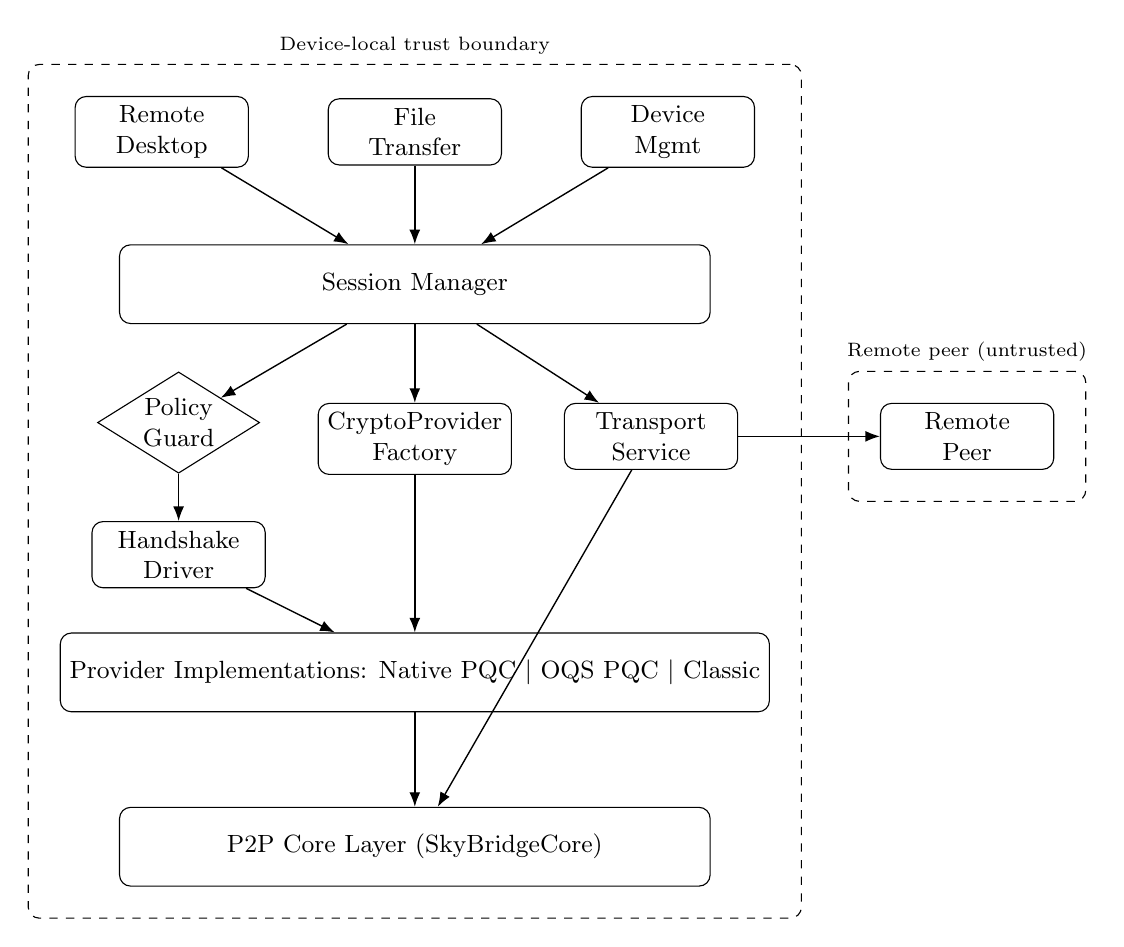
\begin{tikzpicture}[
  font=\small,
  box/.style={draw, rounded corners, align=center, minimum height=8mm, minimum width=22mm},
  layer/.style={draw, rounded corners, align=center, minimum height=10mm, minimum width=75mm},
  guard/.style={draw, diamond, aspect=1.6, align=center, inner sep=1pt, fill=white},
  boundary/.style={draw, dashed, rounded corners, inner sep=4mm},
  arrow/.style={-Latex, line width=0.5pt}
]
  % Top row
  \node[box] (rd) {Remote\\Desktop};
  \node[box, right=10mm of rd] (ft) {File\\Transfer};
  \node[box, right=10mm of ft] (dm) {Device\\Mgmt};

  % Session manager
  \node[layer, below=10mm of ft] (sm) {Session Manager};

  % Core services
  \node[guard, below=6mm of sm, xshift=-30mm] (pg) {Policy\\Guard};
  \node[box, below=6mm of pg] (hd) {Handshake\\Driver};
  \node[box, below=10mm of sm] (cpf) {CryptoProvider\\Factory};
  \node[box, below=10mm of sm, xshift=30mm] (ts) {Transport\\Service};
  \node[box, right=18mm of ts] (rp) {Remote\\Peer};

  % Provider implementations
  \node[layer, below=20mm of cpf] (pi) {Provider Implementations: Native PQC $|$ OQS PQC $|$ Classic};

  % Core module
  \node[layer, below=12mm of pi] (core) {P2P Core Layer (SkyBridgeCore)};

  % Trust boundaries
  \node[boundary, fit=(rd)(ft)(dm)(sm)(pg)(hd)(cpf)(ts)(pi)(core),
    label={[font=\scriptsize]above:Device-local trust boundary}] (local) {};
  \node[boundary, fit=(rp), label={[font=\scriptsize]above:Remote peer (untrusted)}] (remote) {};

  % Arrows
  \draw[arrow] (rd) -- (sm);
  \draw[arrow] (ft) -- (sm);
  \draw[arrow] (dm) -- (sm);

  \draw[arrow] (sm) -- (pg);
  \draw[arrow] (pg) -- (hd);
  \draw[arrow] (sm) -- (cpf);
  \draw[arrow] (sm) -- (ts);

  \draw[arrow] (cpf) -- (pi);
  \draw[arrow] (hd) -- (pi);
  \draw[arrow] (ts) -- (core);
  \draw[arrow] (pi) -- (core);
  \draw[arrow] (ts) -- (rp);
\end{tikzpicture}
\caption{SkyBridge Compass system architecture showing device-local trust
boundary (dashed) and policy guard (diamond).}
\label{fig:architecture}
\end{figure*}

\textbf{Implementation alignment (artifact snapshot, 2026-01-23).} In the
current code revision, connection orchestration for the remote
desktop/file-transfer path is route-aware and authentication-gated:
local discovery can prefer USB-capable host endpoints, control-channel
connections are promoted to ``connected'' only after handshake
authentication, and active file-transfer routing prioritizes live
authenticated sessions before fallback candidates. These implementation
surfaces are enumerated in the Supplementary Artifact Map.

\subsection{CryptoProvider
Protocol}\label{b.-cryptoprovider-protocol}

The CryptoProvider protocol defines a unified interface for all
cryptographic operations required by the handshake and session layers \cite{ref37}.
This abstraction enables transparent substitution of underlying
implementations without modifying caller code.


The \texttt{SigningKeyHandle} abstraction resolves the apparent conflict
between ``private key as Data'' and ``Secure Enclave keys never leave
hardware.'' Software keys are one variant; hardware-backed keys use a
reference or callback, ensuring the protocol interface does not assume
exportability.

The protocol mandates \texttt{Sendable} conformance, ensuring
thread-safe usage across Swift's structured concurrency model. Each
provider exposes its tier classification (\texttt{nativePQC},
\texttt{liboqsPQC}, or \texttt{classic}) and active cipher suite,
enabling runtime introspection for logging and policy enforcement.

\subsection{CryptoSuite Wire
Format}\label{c.-cryptosuite-wire-format}

A \textbf{suite} defines the handshake tuple
\texttt{(KEM,\ SIG,\ AEAD,\ KDF)} used for the KEM-DEM envelope and
transcript binding. Data-plane AEAD is negotiated separately and is
fixed to AES-256-GCM in v1 (Table~\ref{tab:aead-mapping}). Suite identifiers use a compact
16-bit wire ID with reserved ranges for hybrid, PQC, classic, and
experimental suites to enable forward compatibility. The full range
table, encoding rules, and X-Wing notes appear in the Supplementary
Materials (Suite Identifiers and Wire Format). Unknown suite identifiers
are parsed as \texttt{unknown(wireId)} for audit visibility and forward
compatibility; negotiation rejects unknown values if they appear in
\texttt{keyShares} or as \texttt{selectedSuite}.

\subsection{Provider Factory and
Selection}\label{d.-provider-factory-and-selection}

The \texttt{CryptoProviderFactory} implements deterministic provider
selection based on runtime capability detection and policy
configuration:


The selection algorithm proceeds as follows:

\begin{enumerate}\raggedright
\tightlist
\item
  \textbf{Capability Detection:} Query the environment for native PQC
  availability and liboqs presence.
\item
  \textbf{Policy Application:} Match detected capabilities against the
  requested policy.
\item
  \textbf{Provider Instantiation:} Create the appropriate provider
  instance for the detected environment and policy.
\item
  \textbf{Event Emission:} Emit a \texttt{SecurityEvent} recording the
  selection decision.
\end{enumerate}

{\raggedright
For \texttt{preferPQC} policy, the precedence order is
\texttt{ApplePQCProvider} $\rightarrow$ \texttt{OQSPQCProvider} $\rightarrow$
\texttt{ClassicProvider}. This order is deterministic. The
\texttt{requirePQC} policy returns an \texttt{UnavailablePQCProvider}. It
throws on all operations if no PQC implementation is available.\par}

\textbf{Terminology alignment.}
We use two orthogonal knobs: provider selection
(\texttt{preferPQC}/\texttt{requirePQC}) and handshake fallback policy
(\texttt{default}/\texttt{strictPQC}). In our evaluation, \texttt{default}
corresponds to prefer-PQC with evented classic fallback permitted, while
\texttt{strictPQC} requires PQC with either (i) Compliance Mode
(no classic establishment) or (ii) Bootstrap-Assisted Mode
(control-only bootstrap plus mandatory PQC rekey).

\subsection{KEM-DEM Authenticated Encryption
Format}\label{e.-kem-dem-authenticated-encryption-format}

We use a KEM-DEM envelope (KEM $\rightarrow$ HKDF $\rightarrow$ AEAD) as
a compatibility layer when native HPKE is unavailable, binding role and
transcript into the key schedule with explicit length limits for DoS
protection. On Apple 26+ platforms, we use native CryptoKit PQC
primitives (ML-KEM/ML-DSA) within the same envelope to preserve a single
wire format across platforms. Full header/body formats, versioning, and
length limits are provided in the Supplementary Materials (KEM-DEM
Envelope).

\textbf{Why not direct RFC 9180 HPKE everywhere (v1)?}
Three engineering constraints motivate this compatibility layer in v1:
(i) a unified transcript/signature binding surface across mixed
provider stacks, (ii) strict backward compatibility with deployed v1
bridge behavior, and (iii) deterministic parser-level DoS checks before
provider dispatch. When native HPKE is available (Apple 26+), our v2
path uses RFC 9180 HPKE directly; thus the v1 KEM-DEM envelope is
transition code, not a claim of new cryptographic primitive design.



\section{HANDSHAKE STATE
MACHINE}\label{sec:handshake-state-machine}

\subsection{Design Principles}\label{a.-design-principles}

The handshake subsystem addresses three critical requirements:

\begin{enumerate}
\tightlist
\item
  \textbf{Race Condition Prevention:} Concurrent message arrival and
  timeout expiration must not cause double-resume of continuations.
\item
  \textbf{Sensitive Material Protection:} Ephemeral private keys and
  shared secrets must be zeroized on all exit paths.
\item
  \textbf{Observability:} All state transitions and failures must emit
  structured events.
\end{enumerate}

\subsection{Actor-Isolated
Architecture}\label{b.-actor-isolated-architecture}

The \texttt{HandshakeDriver} actor manages handshake state with
compile-time data race prevention:


The \texttt{HandshakeContext} actor isolates sensitive cryptographic
material:


\textbf{Reentrancy Considerations.} Swift actors permit method re-entry
at suspension points (\texttt{await}). While actor isolation prevents
data races, it does not prevent interleaving of method executions. Our
\texttt{HandshakeDriver} mitigates reentrancy risks by routing completion
through \texttt{finishOnce(with:)}, buffering early results, canceling
timeouts on completion, and advancing state before \texttt{await}
points.

\textbf{Await-window limitation.} The
\texttt{handle\allowbreak MessageB} method awaits \texttt{cryptoProvider} operations
inside the actor. If a new message arrives during this await, the actor
could theoretically process it before the current operation completes.
We mitigate this by advancing state to \texttt{.processingMessageB}
before the await, copying immutable inputs, validating a monotonic epoch
counter after resumption, and emitting security events on unexpected
transitions.

This approach provides structural protection against reentrancy hazards
rather than relying on timing assumptions. A formal analysis using model
checking is planned for future work.

\subsection{State Transitions}\label{c.-state-transitions}

Fig.~\ref{fig:state-machines} illustrates the handshake state machine for both roles.

\begin{figure}[!t]
\centering
\resizebox{0.95\columnwidth}{!}{%
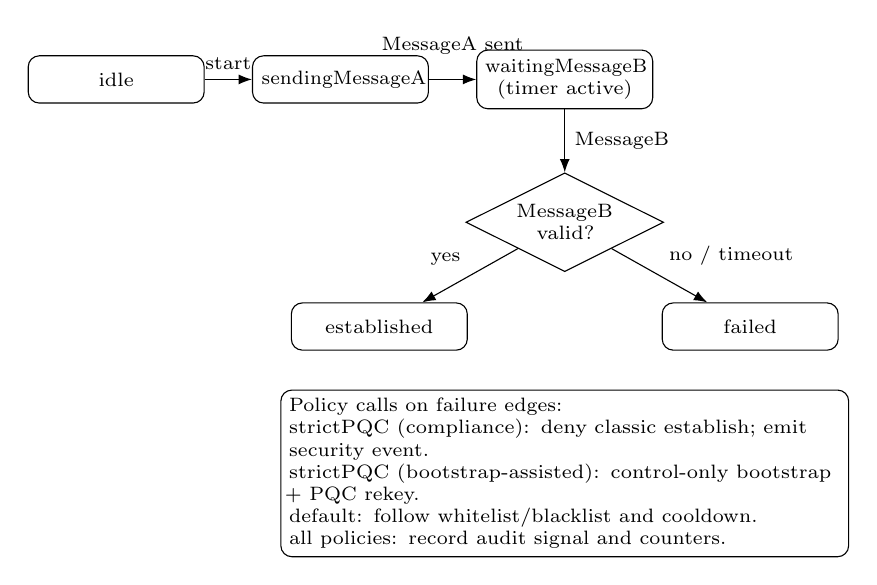
\begin{tikzpicture}[
  font=\scriptsize,
  state/.style={draw, rounded corners, align=center, minimum height=6mm, text width=20mm},
  decision/.style={draw, diamond, aspect=2, align=center, inner sep=1pt, text width=14mm},
  policy/.style={draw, rounded corners, align=left, font=\scriptsize, text width=70mm, inner sep=3pt},
  arrow/.style={-Latex, line width=0.4pt}
]
  \node[state] (i_idle) {idle};
  \node[state, right=6mm of i_idle] (i_send) {sendingMessageA};
  \node[state, right=6mm of i_send] (i_wait) {waitingMessageB\\(timer active)};
  \node[decision, below=8mm of i_wait] (i_dec) {MessageB\\valid?};
  \node[state, below left=7mm and 6mm of i_dec] (i_est) {established};
  \node[state, below right=7mm and 6mm of i_dec] (i_fail) {failed};

  \draw[arrow] (i_idle) -- node[above]{start} (i_send);
  \draw[arrow] (i_send) -- node[above, yshift=2mm]{MessageA sent} (i_wait);
  \draw[arrow] (i_wait) -- node[right]{MessageB} (i_dec);
  \draw[arrow] (i_dec) -- node[above left]{yes} (i_est);
  \draw[arrow] (i_dec) -- node[above right]{no / timeout} (i_fail);

  \coordinate (i_mid) at ($(i_est)!0.5!(i_fail)$);
  \node[policy, below=8mm of i_mid] {
    Policy calls on failure edges:\\
    strictPQC (compliance): deny classic establish; emit security event.\\
    strictPQC (bootstrap-assisted): control-only bootstrap + PQC rekey.\\
    default: follow whitelist/blacklist and cooldown.\\
    all policies: record audit signal and counters.
  };
\end{tikzpicture}%
}

\vspace{2mm}

\resizebox{0.95\columnwidth}{!}{%
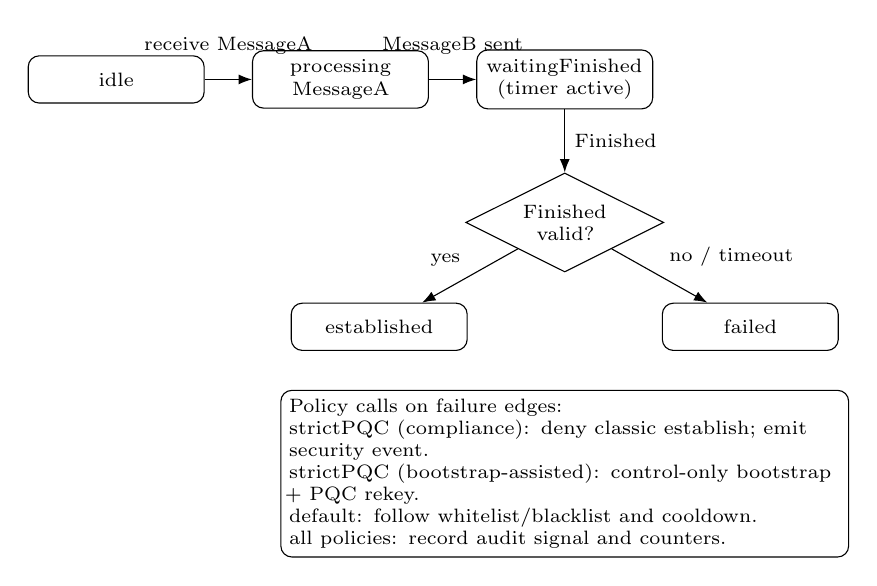
\begin{tikzpicture}[
  font=\scriptsize,
  state/.style={draw, rounded corners, align=center, minimum height=6mm, text width=20mm},
  decision/.style={draw, diamond, aspect=2, align=center, inner sep=1pt, text width=14mm},
  policy/.style={draw, rounded corners, align=left, font=\scriptsize, text width=70mm, inner sep=3pt},
  arrow/.style={-Latex, line width=0.4pt}
]
  \node[state] (r_idle) {idle};
  \node[state, right=6mm of r_idle] (r_proc) {processing\\MessageA};
  \node[state, right=6mm of r_proc] (r_wait) {waitingFinished\\(timer active)};
  \node[decision, below=8mm of r_wait] (r_dec) {Finished\\valid?};
  \node[state, below left=7mm and 6mm of r_dec] (r_est) {established};
  \node[state, below right=7mm and 6mm of r_dec] (r_fail) {failed};

  \draw[arrow] (r_idle) -- node[above, yshift=2mm]{receive MessageA} (r_proc);
  \draw[arrow] (r_proc) -- node[above, yshift=2mm]{MessageB sent} (r_wait);
  \draw[arrow] (r_wait) -- node[right]{Finished} (r_dec);
  \draw[arrow] (r_dec) -- node[above left]{yes} (r_est);
  \draw[arrow] (r_dec) -- node[above right]{no / timeout} (r_fail);

  \coordinate (r_mid) at ($(r_est)!0.5!(r_fail)$);
  \node[policy, below=8mm of r_mid] {
    Policy calls on failure edges:\\
    strictPQC (compliance): deny classic establish; emit security event.\\
    strictPQC (bootstrap-assisted): control-only bootstrap + PQC rekey.\\
    default: follow whitelist/blacklist and cooldown.\\
    all policies: record audit signal and counters.
  };
\end{tikzpicture}%
}
\caption{Handshake state machines for Initiator (top) and Responder
(bottom).}
\label{fig:state-machines}
\end{figure}

\subsection{Double-Resume
Prevention}\label{d.-double-resume-prevention}

The \texttt{finishOnce} method provides a single convergence point for handshake completion, handling the race between timeout expiration and message arrival by: (1) canceling the timeout task on any completion, (2) guarding continuation access with immediate nil assignment, and (3) buffering early results for late continuation establishment.

\subsection{Secure Zeroization}\label{e.-secure-zeroization}

Swift's standard \texttt{Data} and \texttt{Array} types use copy-on-write (COW) semantics, which can leave uncontrolled copies of sensitive material in memory. The \texttt{SecureBytes} class addresses this by using manual \texttt{UnsafeMutableRawPointer} allocation to maintain exclusive ownership, preventing COW-induced secret proliferation. All failure paths explicitly call \texttt{context.zeroize()} before error propagation, with \texttt{deinit} zeroization as defense-in-depth. On Darwin platforms, zeroization uses platform-supported secure wipe primitives (e.g., \texttt{explicit\_bzero} or \texttt{memset\_s}) where available. We avoid exporting secrets as \texttt{Data} when possible, but acknowledge that OS-level snapshots, API boundary copies, or privileged inspection can still retain residues; zeroization is a defense-in-depth measure rather than a sole security boundary.

\subsection{Transcript Binding and Signature
Separation}\label{f.-transcript-binding-and-signature-separation}

The protocol uses domain-separated signatures to prevent cross-message
and cross-session replay attacks.

\textbf{Signature A (MessageA)} is computed by the Initiator over the
MessageA-local fields, binding suite preference, policy intent, and
identity context before any responder data is received:

For Signature A, the initiator signs \texttt{SkyBridge-A}, protocol
version, canonical suite/key-share set, client nonce, capabilities,
policy, and initiator identity key. Optional Secure Enclave binding
uses \texttt{SkyBridge-SE-A}.

\textbf{Signature B (MessageB):} The Responder signs a transcript that
commits to MessageA:

For Signature B, the responder signs \texttt{SkyBridge-B},
\texttt{transcriptA}, selected suite wire ID, responder key share,
server nonce, payload hash, and responder identity key. Optional Secure
Enclave binding uses \texttt{SkyBridge-SE-B}.

\textbf{Key Derivation:} Nonces, transcripts, suite binding, and
\emph{directional separation} are included in the KDF, and the salt is
transcript-bound (non-empty):

KDF input concatenates the \texttt{SkyBridge-KDF} label, suite wire ID,
transcript hashes, and nonces. The salt uses the domain string
\texttt{SkyBridge-KDF-Salt-v1|}. Direction labels separate traffic
classes:
\begin{itemize}
\item \texttt{initiator\_to\_responder}
\item \texttt{responder\_to\_initiator}
\end{itemize}


This structure is designed to ensure: (1) \texttt{sigB} commits to \texttt{MessageA},
so any tampering breaks verification; (2) domain separators prevent
cross-protocol attacks; (3) SE signatures are session-bound and
non-replayable.



\section{SECURITY MODEL AND
GUARANTEES}\label{sec:security-model}

\subsection{Security Model}\label{a.-security-model}

We assume an active network adversary with full control of the discovery
channel (drop, delay, reorder, duplicate, modify, and inject messages)
but without breaking standard cryptographic assumptions. The attacker
can replay prior handshakes and attempt downgrade by suppressing
PQC-related fields. We assume the out-of-band pairing ceremony is
trusted and that device key storage (Keychain/Secure Enclave) preserves
key integrity. The attacker may compromise a peer after pairing and
learn long-term signing key material, but cannot retroactively forge
signatures for past sessions. We do not claim forward secrecy for
KEM-based suites in v1: ML-KEM encapsulation targets a peer's long-term
KEM public key obtained during pairing. Accordingly, post-quantum
confidentiality against store-now-decrypt-later adversaries holds only
while long-term KEM private keys remain uncompromised; later compromise
of the corresponding KEM private key can enable decryption of recorded
sessions.

\textbf{Assumptions:}
\begin{itemize}\tightlist
\item
  The pairing ceremony delivers the correct peer identity key (PIN or
  visual verification is not bypassed).
\item
  Pinned identity keys stored in Keychain/Secure Enclave retain integrity
  across normal device operation.
\item
  Devices remain uncompromised (no root or malware control) during
  handshake execution.
\end{itemize}

\textbf{If assumptions fail:}
\begin{itemize}\tightlist
\item
  If pairing is subverted and the pinned identity key is replaced,
  peer authentication is no longer meaningful; the system must require
  re-pairing and treat the session as untrusted.
\item
  If device integrity is lost, confidentiality and key secrecy cannot be
  guaranteed; the system should abort and emit high-severity events such
  as \texttt{identity}\allowbreak\texttt{Mismatch} or
  \texttt{handshake}\allowbreak\texttt{Failed}.
\end{itemize}

To keep boundary handling operationally explicit, Supplementary
Table~\ref{tab:supp-boundary-stress} enumerates boundary-stress cases
(pairing social engineering, endpoint compromise classes, and audit-log
abuse), their in/out-of-model status, expected event signals, and
required operator actions.

\subsection{Security Goals, Formal Definitions, and Proof
Sketches}\label{b.-security-goals-and-proof-sketches}

\textbf{Definitions.}
\begin{itemize}\tightlist
\item \textbf{D1 (Forced downgrade / forced fallback).} A downgrade occurs if a business-capable session is established with a classic suite when strict policy requires PQC, or if classic fallback is accepted under the default policy without satisfying the local-only fallback gate (Definition D2) and without emitting the corresponding audit event (Property G8).
\item \textbf{D2 (Local-only fallback gate, default policy).} Fallback is permitted only after (i) the peer identity is verified against the pinned key (paired peers) and (ii) the triggering failure is locally generated capability/instantiation unavailability (whitelist), excluding timeout and any unauthenticated network-derived failure.
\item \textbf{D3 (Audit evidence).} The minimal sufficient evidence set is the tuple \{event type, timestamp, deviceId, suiteId, failure reason code, policy mode, fallback flag, cooldown remaining\} (Property G8).
\item \textbf{D4 (Bootstrap-Assisted strict recovery gate).} In strict policy, a temporary classic control channel is allowed only for paired KEM-key recovery triggers (\texttt{missingKEM}, \texttt{staleKEMRecovery}); non-control business messages are blocked until PQC rekey succeeds.
\end{itemize}

\textbf{Lemma L1 (Timeout-triggered fallback impossibility).}
Consider any migration policy that permits classic fallback on timeout or
other unauthenticated network-derived failures. Under the active attacker
model in Section~\ref{sec:security-model} (drop/delay/reorder), the
adversary can force repeated timeout observations on the PQC path and
thereby force classic establishment.
\emph{Proof sketch:} the attacker suppresses or delays PQC-path messages
past the timeout boundary; if timeout is fallback-eligible, each attempt
has a reachable classic edge under attacker control.

\textbf{Corollary C1 (Necessary fallback gate condition).}
To retain compatibility fallback without attacker-forced downgrade,
fallback eligibility must exclude timeout/network-derived failures and be
restricted to attacker-non-inducible local causes (Definition D2), or
classic fallback must be disabled entirely.

We state the core properties as theorem/proposition-level claims tied to
standard assumptions and protocol mechanics. To reduce vacuity risk, the
released Tamarin artifact models explicit classic/PQC/v2 traces, explicit
fallback-gate and downgrade events, and includes existence lemmas in
addition to safety lemmas (\texttt{formal/skybridge\_v2.spthy}) \cite{ref43}.
This revision additionally verifies
timeout-fallback denial, cooldown rate limiting, downgrade-context
evidence, and bootstrap control-only rekey ordering; their
implementation-level traceability anchors are summarized in
Supplementary Table~\ref{tab:supp-formal-code-traceability}.

\textbf{Formal security definitions (experiment style).}
\begin{itemize}\tightlist
\item \textbf{$\mathrm{Exp}_{\mathrm{auth}}$:} adversary wins if it causes a paired endpoint to accept an unauthenticated peer identity.
\item \textbf{$\mathrm{Exp}_{\mathrm{neg}}$:} adversary wins if \texttt{selectedSuite} is accepted outside the signed/advertised offer context.
\item \textbf{$\mathrm{Exp}_{\mathrm{dg}}$:} adversary wins if classic establishment occurs in violation of strict policy, or under default policy without local fallback gate + downgrade event.
\item \textbf{$\mathrm{Exp}_{\mathrm{fs\mbox{-}hybrid}}$:} for v2, adversary wins if it computes session keys without both static KEM contribution and ephemeral contribution under transcript binding.
\end{itemize}

\textbf{Assumption set.}
\begin{itemize}\tightlist
\item KEM IND-CCA security for negotiated KEM suite (ML-KEM/X-Wing profile).
\item Signature EUF-CMA security for protocol signatures (ML-DSA-65 / Ed25519 as configured).
\item HKDF-SHA256 as a PRF in the used extraction/expansion domain.
\end{itemize}

\textbf{Theorem T1 (Authentication).} Under EUF-CMA and trusted pairing pins,
advantage in $\mathrm{Exp}_{\mathrm{auth}}$ is negligible up to bounded
implementation error terms (e.g., policy misconfiguration outside the model).

\textbf{Theorem T2 (Negotiation integrity).} Under EUF-CMA and transcript
binding, advantage in $\mathrm{Exp}_{\mathrm{neg}}$ is negligible.

\textbf{Proposition P1 (Policy-gated downgrade).} Under the threat model in
Section~\ref{sec:security-model}, timeout/drop/reorder adversaries cannot
force successful classic establishment in strict policy, and cannot produce
silent classic fallback in default policy without the local gate event.

\textbf{Proposition P2 (v2 hybrid FS semantics).} For v2 sessions,
compromise of long-term KEM private key alone is insufficient to reconstruct
the derived session root unless the ephemeral contribution secret is also
recovered. This is an intermediate secrecy guarantee and is intentionally
weaker than full ephemeral-ephemeral PFS.

\textbf{Property G1 (Negotiation Integrity):} The selected suite must be
among the Initiator's offered suites and have a corresponding key
share.\\
\emph{Proof sketch:}
\begin{itemize}\tightlist
\item
  \texttt{MessageB} includes \texttt{selectedSuite}, and
  \texttt{sigB} covers \texttt{MessageA}.
\item
  Any modification to the offered suite list or key-share list breaks
  \texttt{sigB} verification.
\item
  The Responder validates \texttt{selectedSuite} against the offered
  suites and checks that a matching key share is present.
\end{itemize}

\textbf{Property G2 (Mutual Authentication for Paired Peers):} For
previously paired devices, the peer identity is authenticated and bound
to the handshake transcript.\\
\emph{Proof sketch:}
\begin{itemize}\tightlist
\item
  \texttt{identityPubKey} is pinned during OOB pairing.
\item
  Signatures in \texttt{MessageA} and \texttt{MessageB} over transcript
  data must verify under the pinned key; otherwise
  \texttt{identityMismatch} aborts the handshake.
\end{itemize}

\textbf{Property G3 (Session Key Secrecy):} The derived session keys
remain secret under standard KEM/DH and signature security
assumptions. For KEM-based PQC suites in v1, we do not claim
post-compromise forward secrecy: confidentiality holds only while
long-term KEM private keys remain uncompromised. In key-control terms,
v1 KEM establishment is initiator-contributory to a responder static
key; v2 adds explicit responder ephemeral contribution to reduce
unilateral key-control concentration.\\
\emph{Proof sketch:}
\begin{itemize}\tightlist
\item
  The shared secret is derived from KEM decapsulation or DH, and keys
  are extracted via HKDF with transcript-bound salt.
\item
  An attacker without the private key material cannot compute the shared
  secret or derive session keys.
\end{itemize}

\textbf{Property G4 (Replay Resistance):} Replayed handshakes do not
establish a session.\\
\emph{Proof sketch:} \texttt{handshakeId} derives from fresh nonces and
suite identifiers; replay detection caches recent IDs and rejects
duplicates within the window.

\textbf{Property G5 (Strict-Policy Consistency):} Strict policy never
permits a business-capable classic session. Compliance Mode has no
classic path. Bootstrap-Assisted Mode may use a transient classic
control channel, but business traffic is blocked until PQC rekey
completes.\\
\emph{Proof sketch:}
\begin{itemize}\tightlist
\item \texttt{TwoAttempt\allowbreak Handshake\allowbreak Manager} enforces a
policy gate before any default-mode fallback attempt.
\item Strict compliance removes classic establishment edges.
\item Strict recovery trigger-limits bootstrap, emits explicit
\texttt{handshake\_fallback} events, and keeps messaging control-only
until PQC rekey succeeds.
\end{itemize}
We validate this behavior using policy downgrade benchmarks
(Fig.~\ref{fig:policy-downgrade}) and bootstrap control-gating tests.

\textbf{Property G6 (Safe Fallback under default policy):} Fallback can
only occur after peer identity is verified under the pinned key and only
for a whitelisted set of locally generated capability errors; timeout
and network-derived failures never trigger fallback.\\
\emph{Proof sketch:} Fallback is gated after identity verification; the
whitelist is evaluated on locally generated capability/instantiation
errors rather than unauthenticated network input. \texttt{timeout} is
explicitly blocked and per-peer cooldown limits repeated downgrades.
\emph{Proposition (No network-induced suiteNegotiation fallback):} Under
Definition D2, \texttt{suiteNegotiationFailed} can trigger
default-mode fallback only in the local pre-send branch (no local
keyshare constructible for the offered PQC suite). If the failure is
observed after remote input, it is treated as network-derived and
cannot satisfy the fallback gate.
\emph{Proposition (No forced fallback by packet loss):} Under the attacker model in Section~\ref{sec:security-model}, an active network attacker who can drop/delay/reorder messages cannot induce a successful classic session by causing timeouts, because timeout-triggered fallback is disallowed and the default-policy fallback gate (Definition D2) requires locally generated unavailability after identity verification.

\textbf{Property G7 (Legacy Acceptance Preconditions):} Legacy P-256
signatures are accepted only under authenticated pairing or an existing
trust record.\\
\emph{Proof sketch:} Legacy acceptance is gated by
\texttt{Legacy\allowbreak Trust\allowbreak Precondition}; pure network stranger connections fail.
This is validated by the precondition test matrix (Table~\ref{tab:legacy-fallback-preconditions}).

\textbf{Property G8 (Auditability):} Cryptographic downgrades and
exceptional states are observable via a minimal sufficient information set.\\
\emph{Proof sketch:} The handshake emits
\texttt{cryptoDowngrade} and related events with reason,
deviceId, and cooldown context, and records them into a per-session
hash-chain (\texttt{AuditTrail}) anchored to the handshake transcript hash,
enabling post-hoc verification of policy adherence and event-order integrity.

\emph{Audit field requirements:}
\begin{itemize}\tightlist
\item \textbf{MUST log} (minimal sufficient set): event type, timestamp, deviceId, suiteId, failure reason code, policy mode, fallback triggered (bool), cooldown remaining.
\item \textbf{MUST NOT log} (privacy preservation): session keys, nonces, raw signatures, message payloads, user identifiers beyond deviceId.
\item \textbf{Tamper-evidence:} In addition to synchronous event emission, each session maintains a transcript-anchored audit hash-chain (\texttt{AuditTrail}). This provides cryptographic tamper evidence for in-session event order/content under non-compromised runtime assumptions. System log retention (\texttt{os\_log}) remains best-effort and can still be truncated by privileged adversaries.
\end{itemize}

\subsection{Complexity and Overhead Bounds}\label{sec:complexity-bounds}

Let $S$ and $K$ denote implementation bounds for offered suites and key
shares (\texttt{maxSupportedSuites}, \texttt{maxKeyShareCount});
currently $S \le 8$ and $K \le 2$. Encoding/decoding work for
MessageA/MessageB is:
\[
T_{\mathrm{codec}} = O(S + K + |M_A| + |M_B|),
\]
with constant-time checks on fixed-length fields and linear passes over
suite/key-share vectors.

Handshake cryptographic operation counts are:
\begin{itemize}\tightlist
\item \textbf{v1 PQC path:} $1\times$ KEM encapsulate + $1\times$ KEM decapsulate + 2 signatures + 2 signature verifies + HKDF key schedule.
\item \textbf{v2 FS path:} v1 counts plus one ephemeral contribution generation per side and one additional shared-secret composition step (HKDF extract-expand on static+ephemeral input).
\item \textbf{Classic path:} one DH-style encapsulation/open path (KEM-DEM abstraction), signatures/verifications, and HKDF key schedule.
\end{itemize}

Closed-form byte overhead between v1 and v2 is dominated by the extra
contribution fields. Let $c_I$ denote the initiator contribution carried
in MessageA and $c_R^{(v1)}, c_R^{(v2)}$ denote responder-share fields
in MessageB for v1 and v2:
\[
\Delta |M_A| = 2 + |c_I|,
\qquad
\Delta |M_B| = |c_R^{(v2)}| - |c_R^{(v1)}|.
\]
In current implementation (\texttt{X25519} contribution, 32 bytes):
$\Delta |M_A| = 34$ bytes and $\Delta |M_B| = 32$ bytes.

\begin{table*}[!t]
\centering
\caption{Security Contract (Properties, Enforcement, Evidence).}
\label{tab:security-contract}
\begin{tabular}{@{}
  >{\raggedright\arraybackslash}p{(\linewidth - 4\tabcolsep) * \real{0.3030}}
  >{\raggedright\arraybackslash}p{(\linewidth - 4\tabcolsep) * \real{0.3939}}
  >{\raggedright\arraybackslash}p{(\linewidth - 4\tabcolsep) * \real{0.3030}}@{}}
\toprule\noalign{}
\begin{minipage}[b]{\linewidth}\raggedright
Property
\end{minipage} & \begin{minipage}[b]{\linewidth}\raggedright
Enforced at
\end{minipage} & \begin{minipage}[b]{\linewidth}\raggedright
Evidence
\end{minipage} \\
\midrule
G1 Negotiation integrity & Suite/keyshare validation + transcript-bound \texttt{sigB} & Fig.~\ref{fig:handshake-sequence}, \mbox{HandshakeDriverTests} \\
G2 Mutual authentication & Identity pinning + signature verification & Table~\ref{tab:failure-mode-robustness} (wrong signature), Table~\ref{tab:legacy-fallback-preconditions} \\
G3 Session key secrecy & KEM/DH + HKDF with transcript-bound salt & Property 1, Supplementary Materials (ML-DSA Key Sizes) \\
G4 Replay resistance & \texttt{handshakeId} cache + nonce binding & Property-Oriented Testing (Section~\ref{sec:evaluation}) \\
G5 Strict-policy consistency & TwoAttempt policy gate + bootstrap control-only gate + mandatory rekey to PQC & Fig.~\ref{fig:policy-downgrade}, \mbox{PolicyDowngradeBenchTests}, \mbox{BootstrapAssuranceTests} \\
G6 Default safe fallback & Whitelist/blacklist + local capability gate + cooldown & Fig.~\ref{fig:downgrade-matrix}, Table~\ref{tab:failure-mode-robustness} \\
G7 Legacy acceptance precondition & LegacyTrustPrecondition & Table~\ref{tab:legacy-fallback-preconditions} \\
G8 Auditability & Security event emission + transcript-anchored \texttt{AuditTrail} hash-chain & Fig.~\ref{fig:failure-histogram}, Table~\ref{tab:audit-signal-fidelity} \\
\bottomrule
\end{tabular}
\end{table*}



\section{Implementation}\label{sec:implementation}

Implementation references (source files, line numbers) are consolidated in the Supplementary Materials (Artifact Map).

\subsection{Platform Support
Matrix}\label{a.-platform-support-matrix}

SkyBridge Compass uses a tiered provider model: a native PQC provider
when available (e.g., CryptoKit ML-KEM/ML-DSA), a portable liboqs
provider, and a classic provider. Provider selection is deterministic
and prefers the strongest available tier; Secure Enclave proof-of-
possession is optional and orthogonal to the negotiated suite. The full
Apple provider matrix and the cross-platform runtime suite-policy matrix
are in the Supplementary Materials (Tables
\ref{tab:supp-platform-support} and \ref{tab:supp-cross-platform-policy}).

\subsection{Native PQC Integration}\label{b.-apple-pqc-integration}

The native provider wraps CryptoKit ML-KEM/ML-DSA APIs \cite{ref1,ref34} when the
SDK exposes them, enabling platform-backed PQC suites and HPKE-based
encapsulation. We treat this as a deployment instance rather than a
protocol dependency; integration details are provided in the
Supplementary Materials (Native PQC Integration).

\subsection{Conditional Compilation
Strategy}\label{c.-conditional-compilation-strategy}

PQC symbols are gated behind build-time flags to keep the codebase
buildable on SDKs that lack PQC types and to avoid compile-time
failures. The flagging strategy and build settings are detailed in the
Supplementary Materials (Conditional Compilation).

\subsection{Security Event
Emission}\label{d.-security-event-emission}

All cryptographic decisions emit structured audit events with
backpressure and rate limiting; implementation details are in the
Supplementary Materials (Security Event Emission).

\subsection{Secure Enclave
Integration}\label{e.-secure-enclave-integration}

For hardware-backed signing, a \texttt{SigningCallback} protocol allows
Secure Enclave keys without exposing private material. Availability,
fallback behavior, and key-type details are provided in the
Supplementary Materials (Secure Enclave Integration).

\subsection{Signing Key Hierarchy}\label{f.-signing-key-hierarchy}

The system uses two complementary signatures: (1) protocol signatures
via the negotiated suite (Ed25519 for classic, ML-DSA-65 for PQC) to bind
peer identity to the transcript, and (2) optional Secure Enclave
P-256 signatures for device proof-of-possession. Protocol signatures are
mandatory; Secure Enclave PoP is optional and provides a hardware-backed
signal. Key hierarchy details and verification rules are provided in the
Supplementary Materials (Signing Key Hierarchy).

\subsection{Pre-Negotiation Signature Algorithm Selection and
Two-Attempt
Strategy}\label{g.-pre-negotiation-signature-algorithm-selection-and-two-attempt-strategy}

A fundamental challenge is that \texttt{sigA} must be generated before
negotiation completes, yet the signature algorithm should match the
negotiated suite. We resolve this with pre-negotiation signature
selection and a two-attempt strategy. Each attempt is homogeneous
(PQC-only or classic-only), and the signature algorithm is chosen based
on the offered suites. The initiator first attempts PQC, then falls back
to classic only for a whitelist of benign, locally generated capability
errors after peer identity verification; timeout, signature
verification, identity mismatch, replay, and other network-derived
failures never trigger fallback. This policy is enforced by the
handshake manager and logged as security events. Detailed error lists
and type-level enforcement are provided in the Supplementary Materials
(Two-Attempt Strategy).
For strict policy deployments, we expose two operator-selectable modes:
\emph{Compliance Mode} (hard fail when PQC cannot be established) and
\emph{Bootstrap-Assisted Mode} (allow one temporary classic control
channel only for paired KEM-key recovery, then require PQC rekey before
business traffic).

\textbf{Fallback Boundary Conditions (Explicit Scope):}
\begin{itemize}\tightlist
\item \emph{We defend against:} (1) Attacker-induced timeout forcing downgrade (blocked by timeout blacklist); (2) Rapid downgrade cycling via repeated failures (5-minute per-peer cooldown); (3) Signature/identity attacks masquerading as capability failures (verification failures are blacklisted).
\item \emph{We do not defend against:} (1) Attacker persistently blocking PQC traffic for $>$5 minutes under default mode (availability vs.\ security trade-off; strict compliance mode provides full protection at cost of connectivity); (2) Legitimate PQC provider failures causing temporary classic fallback under default mode.
\item \emph{Cooldown rationale:} We set a conservative default of 5 minutes to bound downgrade cycling while limiting availability impact; the cooldown is a tunable policy knob. Operators requiring zero classic establishment can select strict Compliance Mode.
\end{itemize}

\begin{table}[!t]
\centering
\scriptsize
\caption{Default-policy fallback classes and remote-inducibility boundary.}
\label{tab:fallback-locality}
\begin{tabular}{@{}
  >{\raggedright\arraybackslash}p{(\linewidth - 4\tabcolsep) * \real{0.47}}
  >{\raggedright\arraybackslash}p{(\linewidth - 4\tabcolsep) * \real{0.53}}@{}}
\toprule
Reason class & Default-policy outcome \\
\midrule
Local capability/instantiation unavailability (pre-send; e.g., local \texttt{suiteNegotiationFailed} due to missing paired KEM keyshare) & ALLOW classic fallback + mandatory \texttt{cryptoDowngrade} event \\
Network-derived / after-send failures (\texttt{timeout}, remote negotiation mismatch, signature/identity/replay failures) & DENY fallback; emit failure event only \\
\bottomrule
\end{tabular}
\end{table}

\textbf{Attempt State and Identifiability:}
\begin{itemize}\tightlist
\item \emph{Shared across attempts:} pinned identity fingerprint and pinned KEM public keys (trust record), and per-peer fallback cooldown state.
\item \emph{Not shared across attempts:} nonces, transcript hashes, handshakeId/replay tags, ephemeral key shares, and session keys; each attempt runs a fresh state machine.
\item \emph{Identifiability:} a passive observer can distinguish a classic fallback attempt from a PQC attempt by wire format. We do not transmit an explicit attempt counter; strict Compliance Mode removes classic attempts entirely when capability privacy outweighs compatibility.
\end{itemize}

\textbf{Security Events:}

Under default policy, classic fallback emits event
``cryptoDowngrade'' with reason, deviceId, and cooldown fields.
Strict Bootstrap-Assisted recovery emits event
``handshake\_fallback'' (bootstrap-assisted mode) with explicit
trigger/result fields. This distinguishes strict compliance
(fail-closed) traces from strict recovery traces with mandatory
PQC rekey.



\section{Evaluation}\label{sec:evaluation}

\subsection{Experimental Setup}\label{a.-experimental-setup}

We evaluate SkyBridge Compass along two primary tracks:
\textbf{security-centric evidence} (fault injection, downgrade
suppression, legacy precondition enforcement, and auditability) and
\textbf{cost-centric evidence} (handshake latency, wire overhead,
provider selection overhead, and data-plane throughput).

\textbf{Environment:} All experiments are run on Apple Silicon (M1/M3 class) with macOS 26.x, where CryptoKit PQC is available when the SDK exposes ML-KEM/ML-DSA types \cite{ref1,ref34}. Build configuration uses Release (\texttt{-O}) with non-essential logging disabled. Timing uses a monotonic clock (\texttt{ContinuousClock}) with 10 warmup runs; per-batch iterations are N=1000 for Classic/liboqs and N=5000 for CryptoKit (stability control). Reported percentiles (p50/p95/p99) are computed directly from samples.

\textbf{Repeatability:} We support multi-batch repeatability by
restarting the benchmark test process for each batch. Supplementary
Tables~\ref{tab:supp-repeatability-latency}--\ref{tab:supp-repeatability-rtt}
report the number of observed batches ($B$) and (when $B \ge 2$) mean and
95\% confidence intervals across batches. To reproduce multi-batch CIs,
re-run the harness with \texttt{SKYBRIDGE\_BENCH\_BATCHES=3}--\texttt{5}.

\textbf{Reproducibility:} We ship an opt-in benchmark suite under \texttt{Tests/\allowbreak SkyBridgeCoreTests/}. For a one-shot run, use \texttt{Scripts/\allowbreak run\_\allowbreak paper\_\allowbreak eval.sh}. The complete command reference and CSV artifact specifications are provided in the Supplementary Materials (Reproducibility).

\textbf{iOS Reproducibility:} We ship an on-device micro-benchmark in
the iOS app (\texttt{Settings} $\rightarrow$ \texttt{PQC} $\rightarrow$
\texttt{Self-test/Bench}) that exports schema-v3 JSON artifacts.
For the pinned run (\texttt{ARTIFACT\_DATE=\artifactdate}), each suite uses
warmup=10, N=1000, and three batches (B=3). We aggregate exported JSON
with \texttt{aggregate\_ios\_microbench.py} into the date-stamped iOS
micro-benchmark CSV, then auto-generate the main table and Supplementary
device metadata. In this frozen run
(iOS/iPadOS 26.2.1), the iOS compatibility-matrix gate passed on both
tested device classes (iPad + iPhone), with no schema or negotiation
incompatibility observed in the benchmark pipeline.

\begin{table*}[!t]
\centering
\caption{On-device micro-benchmark on iOS 26+ (two devices, schema v3 artifacts). Each device runs warmup=10, N=1000, batches=3. Cells report mean/p99 in ms from pooled measured iterations. Data from \texttt{Artifacts/ios\_microbench\_2026-01-23.csv} (generated via \texttt{Scripts/aggregate\_ios\_microbench.py}).}
\label{tab:ios-microbench}
{\setlength{\tabcolsep}{3pt}\scriptsize
\begin{tabular}{@{}lcccccccc@{}}
\toprule
Configuration & \multicolumn{4}{c}{\texttt{ipad16\_3}} & \multicolumn{4}{c}{\texttt{iphone17\_1}} \\
\cmidrule(lr){2-5}\cmidrule(lr){6-9}
& KEM encap & Sign & Verify & KEM-DEM & KEM encap & Sign & Verify & KEM-DEM \\
\midrule
Classic (X25519 + Ed25519) & 0.182 / 7.314 & 0.105 / 0.072 & 0.067 / 0.049 & 0.388 / 7.588 & 0.190 / 7.479 & 0.111 / 0.086 & 0.066 / 0.046 & 0.426 / 8.052 \\
CryptoKit PQC (ML-KEM-768 + ML-DSA-65) & 0.131 / 0.097 & 1.771 / 8.396 & 0.103 / 0.071 & 0.333 / 7.519 & 0.143 / 0.272 & 3.135 / 10.124 & 0.125 / 0.091 & 0.387 / 8.232 \\
CryptoKit Hybrid (X-Wing + ML-DSA-65) & 0.215 / 7.375 & 1.671 / 8.454 & 0.106 / 0.072 & 0.424 / 7.558 & 0.255 / 8.108 & 2.711 / 9.960 & 0.127 / 0.096 & 0.520 / 8.591 \\
\bottomrule
\end{tabular}
}
\end{table*}


\textbf{Interpretation:} Table~\ref{tab:ios-microbench} reports
\emph{primitive-level} iOS costs (encap/sign/verify/seal+open), not
end-to-end handshake completion. It is therefore not interpreted as a
direct substitute for macOS loopback handshake latency.

\subsection{Claim Scope and External Validity}\label{sec:claim-scope-validity}

We separate \emph{mechanism-level} from \emph{deployment-level} claims.
Mechanism-level claims cover negotiation integrity, policy-gated
downgrade behavior, deterministic failure semantics, and audit-event
completeness under the stated threat model. These claims are tied to the
protocol contract and test/formal artifacts, not to Apple-specific APIs.
Deployment-level claims cover absolute latency, wire overhead, and
provider/runtime effects. They are evaluated only for the reported
Apple-platform instance and should not be extrapolated to other OS
stacks without remeasurement. To reduce portability ambiguity, we ship:
\begin{itemize}\tightlist
\item a cross-platform contract-consistency JSON artifact
(Supplementary Table~\ref{tab:supp-cross-platform-contract});
\item a dedicated external Linux direct-path run
(Supplementary Table~\ref{tab:supp-ec2-direct}).
\end{itemize}

Accordingly, we use the real-network results as external-validity
evidence rather than ecosystem-wide performance characterization: the
current snapshot includes one STUN-coupled non-overlay direct path,
overlay-mediated paths, and a dedicated external Linux direct-path run
(\texttt{n=50} per payload), and is used to validate directional
robustness and failure semantics under deployment constraints.

\begin{table*}[!t]
\centering
\scriptsize
\caption{Claim-to-evidence strength map (main-paper claims only).}
\label{tab:claim-evidence-strength}
\begin{tabular}{@{}
  >{\raggedright\arraybackslash}p{(\linewidth - 6\tabcolsep) * \real{0.22}}
  >{\raggedright\arraybackslash}p{(\linewidth - 6\tabcolsep) * \real{0.20}}
  >{\raggedright\arraybackslash}p{(\linewidth - 6\tabcolsep) * \real{0.23}}
  >{\raggedright\arraybackslash}p{(\linewidth - 6\tabcolsep) * \real{0.35}}@{}}
\toprule
Claim axis & Evidence method & Scale / sample scope & Artifact / section anchor \\
\midrule
Negotiation integrity and transcript binding & Formal proof obligations + protocol/property tests & Theorem/Proposition set + reproducible seeded tests & Section~\ref{sec:security-model}; \texttt{formal/skybridge\_v2.spthy}; Section~\ref{sec:evaluation} \\
Policy-gated downgrade correctness & Decision-matrix validation + forced-error policy bench + migration-threat harness contrast & N=1000 per policy/scenario family; Wilson CI reported & Fig.~\ref{fig:policy-downgrade}; Fig.~\ref{fig:downgrade-matrix}; Table~\ref{tab:ablation-by-property}; Table~\ref{tab:migration-threat-harness}; Table~\ref{tab:migration-provider-matrix}; policy-downgrade + migration-threat CSV artifacts \\
Deterministic failure semantics and event typing & Fault injection + spec-to-event trace mapping & Fault injection n=1000 per scenario; MR=1.00/SR=0.00 in reported classes & Table~\ref{tab:failure-mode-robustness}; Table~\ref{tab:audit-signal-fidelity}; fault-injection CSV artifact \\
Performance and overhead characterization & Distributional microbench + system-level amortization & Classic/liboqs N=1000, CryptoKit N=5000; multi-batch CI support & Table~\ref{tab:perf-summary}; Fig.~\ref{fig:system-impact-amortization}; Section~\ref{sec:system-impact} \\
External-validity guardrail (deployment instance) & Controlled simulation + kernel cross-check + fleet-level migration dynamics + real-network micro-study & Controlled N=10{,}000/condition; dedicated direct-path external run n=50/payload & Table~\ref{tab:network-conditions}; Table~\ref{tab:migration-fleet-behavior}; Section~\ref{sec:network-conditions}; Supplementary Tables~\ref{tab:supp-kernel-emulation}, \ref{tab:supp-ec2-direct}, \ref{tab:supp-interop-matrix}; migration-fleet/interoperability CSV artifacts \\
\bottomrule
\end{tabular}
\end{table*}

\textbf{Threats to Validity (Reviewer-facing).}
\emph{Internal validity:} benchmark outcomes can be affected by runtime
noise (scheduler/cache/thermal state), so we use Release builds, warmup,
distributional reporting, and multi-batch restart support.
\emph{Construct validity:} loopback \emph{time-to-ready} and
microbenchmarks are not direct user-perceived QoE, so we report
system-level \texttt{T\_connect}/\texttt{T\_first\_frame}/\texttt{T\_total}
separately and keep these interpretations explicit.
\emph{External validity:} absolute costs are deployment-instance results
(Apple platforms) and are not generalized across ecosystems; cross-stack
evidence is therefore framed as contract-consistency plus targeted Linux
direct-path checks.
\emph{Conclusion validity:} audit-signal ``fidelity'' is a deterministic
spec-to-event conformance check (not statistical classification), and we
publish artifacts for independent reruns.

\subsection{Security Validation}\label{b.-security-centric-evaluation}

We validate security properties through fault injection, property-based
testing, and audit-signal fidelity analysis. This section presents the
key results; detailed test matrices and methodology are provided in the
Supplementary Materials (Regression Testing).

\textbf{Migration-threat harness (baseline contrast).}
To evaluate migration behavior under active suppression, we run a
targeted harness with four metrics:
\textbf{FDR} (forced downgrade rate), \textbf{SDR} (silent downgrade
rate), \textbf{ECR} (evidence completeness rate for emitted downgrade
events), and \textbf{PCR} (policy-decision replayability rate from
recorded traces). We compare a naive timeout-fallback baseline against
SkyBridge policies under a timeout-attack scenario (N=1000).

\begin{table*}[!t]
\centering
\scriptsize
\caption{Migration-threat harness under active timeout suppression (N=1000 per row). Data source: \texttt{Artifacts/\allowbreak migration\_threat\_harness\_\artifactdate.csv} produced by \texttt{MigrationThreatHarnessBenchTests}.}
\label{tab:migration-threat-harness}
\begin{tabular}{@{}
  >{\raggedright\arraybackslash}p{(\linewidth - 12\tabcolsep) * \real{0.19}}
  >{\raggedright\arraybackslash}p{(\linewidth - 12\tabcolsep) * \real{0.11}}
  >{\centering\arraybackslash}p{(\linewidth - 12\tabcolsep) * \real{0.07}}
  >{\centering\arraybackslash}p{(\linewidth - 12\tabcolsep) * \real{0.07}}
  >{\centering\arraybackslash}p{(\linewidth - 12\tabcolsep) * \real{0.07}}
  >{\centering\arraybackslash}p{(\linewidth - 12\tabcolsep) * \real{0.07}}
  >{\raggedright\arraybackslash}p{(\linewidth - 12\tabcolsep) * \real{0.42}}@{}}
\toprule
Configuration & Scenario & FDR & SDR & ECR & PCR & Interpretation \\
\midrule
SkyBridge default & Timeout attack & 0.00 & 0.00 & 1.00 & 1.00 & Timeout does not open classic fallback edge \\
SkyBridge strictPQC & Timeout attack & 0.00 & 0.00 & 1.00 & 1.00 & Compliance mode remains fail-closed under suppression \\
Naive timeout-fallback baseline & Timeout attack & 1.00 & 1.00 & 0.00 & 0.00 & Attacker can force classic with no replayable audit evidence \\
SkyBridge default & Local unavailability & 1.00 & 0.00 & 1.00 & 1.00 & Local-only fallback path is explicit and fully evidenced \\
\bottomrule
\end{tabular}
\end{table*}

This contrast provides implementation-level evidence for Lemma~L1 and
Corollary~C1: timeout-eligible fallback is attacker-forcible, while a
local-only gate removes that adversarial edge.

\textbf{Provider/back-end consistency check (non-Apple path).}
To validate that migration semantics are not tied to Apple-native
providers, we rerun the same harness using explicit liboqs and classic
provider selection. Table~\ref{tab:migration-provider-matrix} reports
the provider-matrix results.

\begin{table*}[!t]
\centering
\scriptsize
\caption{Provider/back-end migration-threat matrix (N=1000 per row). Data source: \texttt{Artifacts/\allowbreak migration\_threat\_provider\_matrix\_\artifactdate.csv} produced by \texttt{MigrationThreatProviderMatrixBenchTests}.}
\label{tab:migration-provider-matrix}
\begin{tabular}{@{}
  >{\raggedright\arraybackslash}p{(\linewidth - 14\tabcolsep) * \real{0.10}}
  >{\raggedright\arraybackslash}p{(\linewidth - 14\tabcolsep) * \real{0.10}}
  >{\raggedright\arraybackslash}p{(\linewidth - 14\tabcolsep) * \real{0.14}}
  >{\centering\arraybackslash}p{(\linewidth - 14\tabcolsep) * \real{0.07}}
  >{\centering\arraybackslash}p{(\linewidth - 14\tabcolsep) * \real{0.07}}
  >{\centering\arraybackslash}p{(\linewidth - 14\tabcolsep) * \real{0.07}}
  >{\centering\arraybackslash}p{(\linewidth - 14\tabcolsep) * \real{0.07}}
  >{\raggedright\arraybackslash}p{(\linewidth - 14\tabcolsep) * \real{0.38}}@{}}
\toprule
Provider & Policy & Scenario & FDR & SDR & ECR & PCR & Interpretation \\
\midrule
liboqs & default & timeout attack & 0.00 & 0.00 & 1.00 & 1.00 & Timeout suppression does not create a classic edge \\
liboqs & strictPQC & timeout attack & 0.00 & 0.00 & 1.00 & 1.00 & Strict mode remains fail-closed under timeout suppression \\
liboqs & default & local unavailability & 1.00 & 0.00 & 1.00 & 1.00 & Local whitelist fallback is explicit and fully evidenced \\
classic & default & PQC provider unavailable & 1.00 & 0.00 & 1.00 & 1.00 & No-PQC backend path still emits replayable downgrade evidence \\
\bottomrule
\end{tabular}
\end{table*}

\textbf{Fleet-level migration dynamics (heterogeneous capability mix).}
To quantify migration behavior beyond per-handshake microbenchmarks, we
run a controlled fleet simulation with heterogeneous peer capability
ratios, per-peer cooldown on/off ablation, and active timeout
suppression (N=10{,}000 sessions per row; peer pool=2{,}000; timeout
attack rate=5\%). Table~\ref{tab:migration-fleet-behavior} reports
availability, downgrade exposure, and policy-decision distribution from
\texttt{Artifacts/\allowbreak migration\_fleet\_behavior\_\artifactdate.csv}.

\begin{table*}[!t]
\centering
\scriptsize
\caption{Fleet-level migration dynamics under heterogeneous PQC capability distributions (N=10{,}000 sessions per row).}
\label{tab:migration-fleet-behavior}
\begin{tabular}{@{}
  >{\centering\arraybackslash}p{(\linewidth - 10\tabcolsep) * \real{0.10}}
  >{\centering\arraybackslash}p{(\linewidth - 10\tabcolsep) * \real{0.10}}
  >{\centering\arraybackslash}p{(\linewidth - 10\tabcolsep) * \real{0.11}}
  >{\centering\arraybackslash}p{(\linewidth - 10\tabcolsep) * \real{0.14}}
  >{\centering\arraybackslash}p{(\linewidth - 10\tabcolsep) * \real{0.12}}
  >{\raggedright\arraybackslash}p{(\linewidth - 10\tabcolsep) * \real{0.43}}@{}}
\toprule
PQC-capable ratio & Cooldown & Success rate & Downgrade events / 1k & Mean connect (ms) & Decision-share breakdown (PQC / classic / rate-limited / timeout) \\
\midrule
20\% & on  & 0.3830 & 195.60 & 0.009 & 0.1874 / 0.1956 / 0.6066 / 0.0104 \\
20\% & off & 0.9899 & 799.80 & 0.010 & 0.1901 / 0.7998 / 0.0000 / 0.0101 \\
50\% & on  & 0.6589 & 185.70 & 0.006 & 0.4732 / 0.1857 / 0.3170 / 0.0241 \\
50\% & off & 0.9761 & 500.80 & 0.007 & 0.4753 / 0.5008 / 0.0000 / 0.0239 \\
80\% & on  & 0.8867 & 124.80 & 0.004 & 0.7619 / 0.1248 / 0.0733 / 0.0400 \\
80\% & off & 0.9595 & 204.80 & 0.005 & 0.7547 / 0.2048 / 0.0000 / 0.0405 \\
\bottomrule
\end{tabular}
\end{table*}

The fleet-level \texttt{mean connect} metric is an in-process
policy/attempt completion cost (not external network RTT) and is reported
only to compare policy modes under identical harness conditions.

\textbf{Failure-Mode Robustness.}
The actor-isolated handshake driver targets deterministic failure semantics; in our fault-injection tests we observed no unhandled errors, double-resume, or sensitive-material leaks. We inject faults including timeout, malformed framing, invalid signatures, out-of-order delivery, and concurrent cancellation (n=1000 per scenario per policy).

\textbf{Unknown-suite handling:} We parse unknown suite identifiers as an
explicit \texttt{unknown(wireId)} value and reject them if they appear in
\texttt{keyShares} or as \texttt{selectedSuite}. This prevents silent
``unknown $\rightarrow$ classic'' coercions that would otherwise weaken
downgrade guarantees.

\begin{table*}[!t]
\centering
\caption{Failure-Mode Robustness and Observability. Runs = number of
iterations per scenario and policy (n=1000). Table reports default
policy; strictPQC (Compliance Mode) counts are recorded separately in
\texttt{fault\_injection\_\artifactdate.csv}. All
metrics are binary (1 = pass) except event counts. Data from
\texttt{Artifacts/fault\_injection\_\artifactdate.csv}
produced by \mbox{HandshakeFaultInjectionBenchTests}; semantic checks from
\mbox{HandshakeDriverTests}.}
\label{tab:failure-mode-robustness}
\begin{tabular}{@{}
  >{\raggedright\arraybackslash}p{(\linewidth - 12\tabcolsep) * \real{0.1186}}
  >{\raggedright\arraybackslash}p{(\linewidth - 12\tabcolsep) * \real{0.0508}}
  >{\raggedright\arraybackslash}p{(\linewidth - 12\tabcolsep) * \real{0.0763}}
  >{\raggedright\arraybackslash}p{(\linewidth - 12\tabcolsep) * \real{0.1356}}
  >{\raggedright\arraybackslash}p{(\linewidth - 12\tabcolsep) * \real{0.1780}}
  >{\raggedright\arraybackslash}p{(\linewidth - 12\tabcolsep) * \real{0.2203}}
  >{\raggedright\arraybackslash}p{(\linewidth - 12\tabcolsep) * \real{0.2203}}@{}}
\toprule\noalign{}
\begin{minipage}[b]{\linewidth}\raggedright
Failure Mode
\end{minipage} & \begin{minipage}[b]{\linewidth}\raggedright
Runs
\end{minipage} & \begin{minipage}[b]{\linewidth}\raggedright
No\\Unexp.\\Error
\end{minipage} & \begin{minipage}[b]{\linewidth}\raggedright
No\\Double\\Resume
\end{minipage} & \begin{minipage}[b]{\linewidth}\raggedright
Zero\\Verified
\end{minipage} & \begin{minipage}[b]{\linewidth}\raggedright
$E_{\texttt{handshakeFailed}}$
\end{minipage} & \begin{minipage}[b]{\linewidth}\raggedright
$E_{\texttt{cryptoDowngrade}}$
\end{minipage} \\
\midrule
Out-of-order & 1000 & 1 & 1 & 1 & 0 & 0 \\
Duplicate & 1000 & 1 & 1 & 1 & 0 & 0 \\
Drop & 1000 & 1 & 1 & 1 & 1000 & 0 \\
Delay within timeout & 1000 & 1 & 1 & 1 & 0 & 0 \\
Delay exceed timeout & 1000 & 1 & 1 & 1 & 1000 & 0 \\
Corrupt header & 1000 & 1 & 1 & 1 & 1000 & 0 \\
Corrupt payload & 1000 & 1 & 1 & 1 & 1000 & 0 \\
Wrong signature & 1000 & 1 & 1 & 1 & 1000 & 0 \\
Concurrent cancel & 1000 & 1 & 1 & 1 & 1000 & 0 \\
Concurrent timeout & 1000 & 1 & 1 & 1 & 1000 & 0 \\
\bottomrule
\end{tabular}
\end{table*}

The delay-within-timeout and delay-exceed-timeout scenarios approximate
RTT jitter and loss-induced stalls, while drop and duplicate cases
approximate packet loss and reordering. The per-scenario event
distributions are recorded in \texttt{Artifacts/\allowbreak fault\_injection\_\allowbreak \artifactdate.csv}.

Downgrade events are quantified separately in the policy bench (Fig.~\ref{fig:policy-downgrade})
to avoid conflating fallback behavior with transport corruption
scenarios.

\begin{figure}
\centering
\pandocbounded{
\includegraphics[keepaspectratio,width=\columnwidth]{figures/fig_policy_downgrade.pdf}}
\caption{Policy guard enforces strictPQC Compliance Mode: fallback events per
1000 runs, macOS 26.x, N=1000 per policy. Error bars show 95\% Wilson binomial CI.}
\label{fig:policy-downgrade}
\end{figure}

The plot in Fig.~\ref{fig:policy-downgrade} uses the policy-downgrade
dataset. File: \texttt{policy\_downgrade\_\artifactdate.csv}. It
demonstrates that strictPQC Compliance Mode never emits fallback events even under
forced PQC-unavailable errors; default policy shows non-zero downgrade
events.

\begin{figure}
\centering
\pandocbounded{
\includegraphics[keepaspectratio,width=\columnwidth]{figures/fig_downgrade_matrix.pdf}}
\caption{Downgrade decision matrix (policy $\times$ error) with
explicit allow/deny semantics, macOS 26.x. Each cell is labeled ALLOW or DENY for grayscale readability.}
\label{fig:downgrade-matrix}
\end{figure}

Fig.~\ref{fig:downgrade-matrix} encodes the explicit downgrade whitelist/blacklist: only
PQC-unavailability and local pre-send suite-selection errors may fallback
under default policy; strictPQC Compliance Mode denies classic fallback edges
(Bootstrap-Assisted strict recovery is a separate control-only path with
mandatory PQC rekey).

\begin{figure}
\centering
\pandocbounded{
\includegraphics[keepaspectratio,width=\columnwidth]{figures/fig_failure_histogram.pdf}}
\caption{Failure-mode histogram of security events, macOS 26.x,
N=1000 per scenario.}
\label{fig:failure-histogram}
\end{figure}

Fig.~\ref{fig:failure-histogram} combines fault-injection counts with the downgrade-acceptance
event from the policy bench to visualize observability of failures and
downgrades across policy modes.

\textbf{\mbox{Property-Oriented} Testing.}
Correctness properties are validated with property-based tests using a
reproducible seed (0xDEADBEEF):
\begin{itemize}\tightlist
\item KEM-DEM round-trip correctness across all providers (100 trials)
\item Signature verification integrity (100 payloads per provider)
\item Secure zeroization on deallocation
\item State-machine single-resume guarantee under concurrent stress
(500 iterations)
\end{itemize}
A standalone Python decoder
(\texttt{Scripts/\allowbreak wire\_\allowbreak format\_\allowbreak sanity.py}) provides non-Swift
interoperability validation of wire formats.

\textbf{ML-DSA Key Lifecycle.}
ML-DSA-65 key generation, storage, and sign/verify operations are
validated against FIPS 204 \cite{ref16}. Size-compliance results are
reported in the Supplementary Materials (ML-DSA Key Sizes). All property
tests (round-trip, tampering detection, key independence) achieve
100\% pass rate. Keys are stored in Keychain with device-local
accessibility and synchronization disabled
(\texttt{kSecAttrSynchronizable=\allowbreak false}).

\textbf{Legacy Fallback Security.}
Legacy P-256 signatures are only accepted when a security precondition is satisfied: (1) authenticated out-of-band channel (QR code, PAKE/PIN), or (2) existing TrustRecord with \texttt{legacyP256PublicKey}. Pure network stranger connections are rejected to prevent downgrade attacks.

\begin{table*}[!t]
\centering
\caption{Legacy Fallback Precondition Test Results. All tests executed
via \mbox{LegacyFallbackPreconditionTests}. Tests validate Property G7: Legacy
Fallback Security Precondition.}
\label{tab:legacy-fallback-preconditions}
\begin{tabular}{@{}
  >{\raggedright\arraybackslash}p{(\linewidth - 6\tabcolsep) * \real{0.1786}}
  >{\raggedright\arraybackslash}p{(\linewidth - 6\tabcolsep) * \real{0.2500}}
  >{\raggedright\arraybackslash}p{(\linewidth - 6\tabcolsep) * \real{0.3036}}
  >{\raggedright\arraybackslash}p{(\linewidth - 6\tabcolsep) * \real{0.2679}}@{}}
\toprule\noalign{}
\begin{minipage}[b]{\linewidth}\raggedright
Scenario
\end{minipage} & \begin{minipage}[b]{\linewidth}\raggedright
Precondition
\end{minipage} & \begin{minipage}[b]{\linewidth}\raggedright
Expected Result
\end{minipage} & \begin{minipage}[b]{\linewidth}\raggedright
Actual Result
\end{minipage} \\
\midrule
Pure network stranger & None & Reject & OK Reject \\
QR code pairing (verified) & authenticatedChannel & Allow & OK Allow \\
PAKE pairing (verified) & authenticatedChannel & Allow & OK Allow \\
Existing TrustRecord with legacy key & existingTrustRecord & Allow & OK Allow \\
Existing TrustRecord without legacy key & None & Reject & OK Reject \\
Network discovery & None & Reject & OK Reject \\
Unverified authenticated channel & None & Reject & OK Reject \\
\bottomrule
\end{tabular}
\end{table*}

\textbf{Property G7 (Legacy Fallback Security Precondition):} A legacy
P-256 signature SHALL only be accepted when a security precondition is
satisfied. Pure network stranger connections SHALL be rejected.
Validated with 12 test cases covering all precondition combinations (100\% coverage of the precondition state space).

\textbf{Audit-Signal Fidelity.}
Security events provide deterministic, audit-friendly (best-effort, non-cryptographic) telemetry of failures and policy decisions. Fig.~\ref{fig:event-traces} illustrates a representative timeout trace showing attacker action, policy gate response, and emitted event.

\emph{Evaluation approach:} We evaluate audit-signal fidelity using a spec-to-event mapping consistency metric, \emph{not} a statistical classifier. Each fault-injection scenario deterministically maps to exactly one expected trace template (event sequence), e.g., timeout $\rightarrow$ \texttt{handshakeFailed=1, cryptoDowngrade=0}. Match rate (MR)=1.00 means all N iterations matched the expected template; spurious rate (SR)=0.00 means no unexpected events were emitted. This is regression consistency against the protocol specification, not ML classification performance.

Table~\ref{tab:audit-signal-fidelity} summarizes results across all fault-injection scenarios: all scenario classes achieve 1.00 match and 0.00 spurious rates, confirming correct event semantics.

\begin{figure}
\centering
\pandocbounded{
\includegraphics[keepaspectratio,width=\columnwidth]{figures/fig_event_traces.pdf}}
\caption{Audit-signal event trace (representative timeout case)
showing attacker action, policy gate, and emitted event.}
\label{fig:event-traces}
\end{figure}

\begin{table*}[!t]
\centering
\caption{Audit-Signal Fidelity Summary. Match/spurious rates reflect \emph{deterministic} protocol event mapping (each scenario maps to exactly one expected trace template), not statistical classification. Perfect scores indicate regression consistency against the protocol specification.}
\label{tab:audit-signal-fidelity}
\begin{tabular}{@{}lllcc@{}}
\toprule
Scenario Class & Expected Signal & N & Match (MR) & Spurious (SR) \\
\midrule
Drop/Timeout (default) & handshakeFailed=1, cryptoDowngrade=0 & 3000 & 1.00 & 0.00 \\
Drop/Timeout (strictPQC) & handshakeFailed=1, cryptoDowngrade=0 & 3000 & 1.00 & 0.00 \\
Corrupt/Wrong Sig & handshakeFailed=1, cryptoDowngrade=0 & 6000 & 1.00 & 0.00 \\
Ordering Benign & handshakeFailed=0, cryptoDowngrade=0 & 6000 & 1.00 & 0.00 \\
PQC unavailable (default) & cryptoDowngrade=1 & 1000 & 1.00 & 0.00 \\
PQC unavailable (strictPQC) & cryptoDowngrade=0 & 1000 & 1.00 & 0.00 \\
\bottomrule
\end{tabular}
\end{table*}

Due to space constraints, the complete regression test matrix, TLV encoding validation, and implementation component details are provided in the Supplementary Materials (Regression Testing and Artifact Map).

\subsection{Resource Amplification and Throttling}\label{sec:resource-amplification}

We separate adversarial cost vectors into (i) pre-authentication parser
cost and (ii) post-authentication retry/cooldown pressure. Pre-auth
cost is bounded by strict field-length checks, overflow-safe parsing, and
bounded key-share cardinality before cryptographic operations are
invoked. Post-auth pressure is bounded by per-peer fallback cooldown and
rate-limited security event emission.

These controls are intended to bound resource amplification from malformed
inputs and retry storms without introducing silent downgrade paths. We do
not claim Internet-scale saturation resistance from this revision alone;
adversarial burst-throughput characterization remains future work.

\subsection{Performance Benchmarks}\label{c.-cost-centric-evaluation}

Table~\ref{tab:perf-summary} consolidates all performance metrics. We measure \mbox{end-to-end} handshake completion time using an in-memory loopback transport to isolate cryptographic and state-machine overhead. Each configuration reports distributional statistics after 10 warmup runs (Classic/liboqs: N=1000; CryptoKit: N=5000).

% Auto-generated by make_tables.py on 2026-02-19T23:17:44.253885
% DO NOT EDIT MANUALLY - regenerate from CSV artifacts

\begin{table*}[!t]
\centering
\caption{Performance Summary. All benchmarks on Apple Silicon (M1/M3), macOS 26.x, configuration-specific N after 10 warmup runs (Classic=1000, liboqs PQC=1000, CryptoKit PQC=5000). Wire Size counts payload-only handshake bytes (MessageA + MessageB + 2$\times$Finished); loopback wire sizes including transport overhead are reported separately in Table~\ref{tab:baseline-comparison} and Supplementary Table~\ref{tab:supp-loopback-wire}. Data-plane AEAD is fixed to AES-256-GCM in v1, so throughput is independent of the negotiated handshake suite; throughput measured post-handshake on 1~MiB payloads.}
\label{tab:perf-summary}
\begin{tabular}{@{}lcccccc@{}}
\toprule
Configuration & \multicolumn{2}{c}{Handshake Latency} & \multicolumn{2}{c}{RTT} & Wire Size & Throughput \\
\cmidrule(lr){2-3} \cmidrule(lr){4-5}
 & mean (ms) & p95 (ms) & p50 (ms) & p95 (ms) & (bytes) & (GB/s) \\
\midrule
Classic & 2.40 & 2.62 & 0.52 & 0.58 & 687 & 3.7 \\
liboqs PQC & 2.95 & 3.69 & 0.89 & 1.45 & 12,002 & 3.7 \\
CryptoKit PQC & 5.33 & 6.22 & 2.06 & 2.78 & 12,009 & 3.7 \\
\bottomrule
\end{tabular}
\end{table*}

\textbf{v1/v2 Bridge Overhead.}
To isolate the protocol-v2 cost, we run a controlled liboqs v1/v2 bridge
comparison with identical hardware/runtime settings (N=1000, warmup=10).
Supplementary Table~\ref{tab:supp-v2-v1-compare} reports mean/p95 latency,
RTT, and payload-handshake bytes. Consistent with the wire-format analysis in
Section~\ref{sec:complexity-bounds}, v2 adds a fixed +\claimVTwoDeltaPayloadBytes~B payload-handshake
overhead (MessageA +\claimVTwoDeltaMessageABytes~B, MessageB +\claimVTwoDeltaMessageBBytes~B), while latency impact remains in the
low-millisecond range.

\textbf{Latency Distribution.}
Fig.~\ref{fig:handshake-latency} shows latency percentiles across
configurations. Classic handshakes remain near
\claimClassicMeanMs~ms (\claimClassicPNineNineMs~ms at p99). CryptoKit
PQC remains around \claimCryptoKitPNineNineMs~ms at p99, with variance
dominated by ML-DSA signature verification overhead. Extended statistics
(mean/p50/p95/p99, std) are
available in Supplementary Tables~\ref{tab:supp-latency}--\ref{tab:supp-rtt}
(reported in the supplementary PDF).

\begin{figure}
\pandocbounded{{\centering
\includegraphics[keepaspectratio,width=\columnwidth]{figures/fig_handshake_latency.pdf}\par}}
\caption{Handshake latency percentiles for Classic, liboqs PQC, and CryptoKit PQC (warmup=10; N=1000 for Classic/liboqs, N=5000 for CryptoKit). Data source: \texttt{handshake\_bench\_\artifactdate.csv}. Values align with Table~\ref{tab:perf-summary} and Supplementary Table~\ref{tab:supp-latency}.}
\label{fig:handshake-latency}
\end{figure}

\textbf{Wire-Format Breakdown.}
The handshake payload size increases from Classic (\claimClassicPayloadBytes~B) to PQC (\claimLiboqsPayloadBytes~B), dominated by ML-DSA signatures (3309~B) and ML-KEM ciphertexts (1088~B). Fig.~\ref{fig:message-size-breakdown} shows the per-field breakdown.
\textbf{Path-MTU implication.}
The payload-only PQC handshake (\claimLiboqsPayloadBytes~B) spans
multiple transport segments under common MTUs. In our design, handshake
messages run over stream transports (TCP/QUIC stream), so
segmentation/reassembly is delegated to transport rather than custom
handshake-layer fragmentation; the practical risk is latency inflation on
lossy paths, which is why we report controlled impairment, kernel-level,
and real-network evidence in Section~\ref{sec:network-conditions}.

\begin{figure}
\pandocbounded{{\centering
\includegraphics[keepaspectratio,width=\columnwidth]{figures/fig_message_size_breakdown.pdf}\par}}
\caption{Handshake message size breakdown (signature, keyshare, identity
fields, framing overhead) for MessageA/MessageB across Classic and PQC
configurations. Counts reflect MessageA/B payloads only. The
\emph{payload-only} handshake size adds two 38~B Finished frames
(accounted for in Table~\ref{tab:perf-summary}); detailed field sizes are
reported in Supplementary Table~\ref{tab:supp-message-sizes}. Data source:
\texttt{message\_sizes\_\artifactdate.csv}.}
\label{fig:message-size-breakdown}
\end{figure}

Note: In the \texttt{2026-01-23} snapshot, X-Wing hybrid KEM adds
128~B to MessageA's keyshare (1216~B vs 1088~B for ML-KEM-768). Measured
handshake sizes are reported in Supplementary
Table~\ref{tab:supp-message-sizes}
(\texttt{MessageA.XWing}/\texttt{MessageB.XWing}).

\textbf{Data-Plane and Provider Selection.}
Post-handshake symmetric AEAD (AES-256-GCM) throughput reaches 3.7~GB/s for 1~MiB payloads on Apple Silicon, with CPU cost of 0.25~ns/byte. In v1 the data-plane AEAD is fixed to AES-256-GCM and recorded separately from the handshake suite; thus throughput is independent of the negotiated KEM/signature suite. Provider selection overhead is sub-microsecond for cached paths (0.17~$\mu$s p50) and under 6~$\mu$s even for fallback scenarios. Detailed breakdowns are provided in the artifact CSV files.

\subsection{System-level Impact and Amortization}\label{sec:system-impact}
The preceding microbenchmarks isolate handshake and cryptographic costs.
To align evaluation with the \emph{remote desktop / file transfer} framing,
we additionally measure user-visible, session-level metrics and quantify
how one-time handshake cost amortizes over longer sessions and larger
transfers.

\textbf{Metrics:}
(i) \texttt{T\_connect} (connect start $\rightarrow$ handshake established, including explicit Finished key confirmation and event emission),
(ii) \texttt{T\_first\_frame} (connect start $\rightarrow$ first decrypted remote-desktop frame processed by the rendering path), and
(iii) \texttt{T\_total} (connect start $\rightarrow$ completion of a bulk transfer over the negotiated session keys).

\textbf{Method:}
We reuse the production \texttt{HandshakeDriver} and negotiated
\texttt{SessionKeys}, with the following setup:
\begin{itemize}\tightlist
\item Workload: one encrypted ``first frame'' plus bulk transfer
workloads (1--100~MiB).
\item Channel model: deterministic RTT+jitter on a reliable stream.
\item Throughput control: bulk payloads are rate-limited
(MiB/s) to avoid per-chunk RTT artifacts.
\item Output: date-stamped system-impact CSV artifact generated by
\texttt{SystemImpactBenchTests}.
\end{itemize}

% Auto-generated by make_tables.py on 2026-02-19T23:17:44.297249
% DO NOT EDIT MANUALLY - regenerate from CSV artifacts
% Source: system_impact_2026-01-23.csv

\begin{table*}[!t]
\centering
\caption{System-level impact and amortization (p50/p95, ms). $T_{connect}$ is measured from connect start to handshake established (including Finished key confirmation and event emission). $T_{total}$ is measured from connect start to completion of an encrypted bulk transfer. Network conditions emulate deterministic RTT+jitter on a reliable stream; large data-plane payloads are bandwidth-limited (MiB/s) to avoid per-chunk RTT artifacts. Runs: $N_{connect}$=1000; $N_{total}$ (RTT 50$\pm$20 ms) = 1MiB:N=1000, 10MiB:N=500, 100MiB:N=100. Data from \texttt{Artifacts/system\_impact\_2026-01-23.csv}.}
\label{tab:system-impact}
\small
\begin{tabular}{@{}lcccccc@{}}
\toprule
& \multicolumn{3}{c}{\textbf{$T_{connect}$ (p50/p95)}} & \multicolumn{3}{c}{\textbf{$T_{total}$ (p50/p95), RTT 50$\pm$20 ms}} \\
\cmidrule(lr){2-4} \cmidrule(lr){5-7}
\textbf{Suite} & ideal & RTT 50$\pm$20 ms & RTT 100$\pm$50 ms & 1 MiB & 10 MiB & 100 MiB \\
\midrule
\textbf{Classic} & 11.9/12.2 & 191.9/198.6 & 407.8/414.6 & 378.3/395.6 & 634.8/657.3 & 3179/3206 \\
\textbf{liboqs PQC} & 14.0/15.1 & 195.1/202.1 & 415.4/430.9 & 372/410 & 638.4/672.6 & 3192/3583 \\
\textbf{CryptoKit PQC} & 16.3/18.4 & 196.2/205.8 & 412.1/426.8 & 371/434 & 581.0/593.2 & 3208/3285 \\
\bottomrule
\end{tabular}
\end{table*}

\begin{figure}
\pandocbounded{{\centering
\includegraphics[keepaspectratio,width=\columnwidth]{figures/fig_system_impact_amortization.pdf}\par}}
\caption{System-level impact and amortization (p95). Top: \texttt{T\_connect} across RTT+jitter conditions. Bottom: total session time (\texttt{T\_total} = connect + transfer) versus file size under RTT 50$\pm$20~ms, showing that one-time handshake overhead is amortized by larger transfers. Data from \texttt{Artifacts/system\_impact\_\artifactdateSystemImpact.csv}.}
\label{fig:system-impact-amortization}
\end{figure}

\textbf{Traffic Analysis Mitigation (SBP2 Padding).}
To reduce attempt identifiability on the wire, SkyBridge optionally applies a constant-size framing layer (SBP2) that buckets framed payloads into powers-of-two-sized envelopes. Here, \textbf{SBP1} denotes \emph{handshake-frame padding} (MessageA/MessageB/Finished are padded to fixed buckets before transport), while \textbf{SBP2} denotes \emph{traffic framing and padding} applied to all framed payloads (control and encrypted data-plane) with a per-frame header and bucketed padding up to a configured cap.
We measure SBP2 behavior on a real protocol trace: an end-to-end handshake (SBP1 + SBP2 enabled) on an in-memory loopback transport, followed by bidirectional AES-GCM--encrypted data-plane frames derived from the negotiated session keys. Supplementary Table~\ref{tab:supp-traffic-padding} reports the resulting quantization behavior and overhead; the full per-label bucket histograms are included in \texttt{Artifacts/\allowbreak traffic\_\allowbreak padding\_\allowbreak \artifactdate.csv}.

\begin{figure}
\pandocbounded{{\centering
\includegraphics[keepaspectratio,width=\columnwidth]{figures/fig_traffic_padding_overhead.pdf}\par}}
\caption{SBP2 padding overhead across representative handshake, control, and data-plane workloads (macOS 26.x). Overhead is computed as \((\texttt{paddedBytes}/\texttt{rawBytes}-1)\times100\%\) aggregated per label over a deterministic trace (N=1000 handshake iterations; data-plane workload uses encrypted control messages and large-frame mixes). Generated from \texttt{Artifacts/\allowbreak traffic\_\allowbreak padding\_\allowbreak \artifactdate.csv}.}
\label{fig:traffic-padding-overhead}
\end{figure}

\textbf{Sensitivity Study (Bucket Cap).}
We vary the maximum bucket size for SBP2 (\emph{cap} = 64\,KiB, 128\,KiB, 256\,KiB) and re-run the same deterministic protocol trace. We report two overhead definitions:
\emph{all-frames overhead} (includes passthrough frames) and
\emph{padded-only overhead} (restricted to frames that entered bucket
padding), alongside \emph{over-cap rate} (fraction of frames whose framed
payload exceeds cap) and \emph{bucket entropy} (Shannon entropy of padded
bucket sizes per label). When over-cap is high, all-frames overhead may
approach zero while padded-only overhead remains non-zero; this is a cap
tradeoff, not a measurement bug. Supplementary
Table~\ref{tab:supp-traffic-padding-sensitivity} summarizes this
overhead--privacy tradeoff and distinguishes remote-desktop-like vs
file-chunk-like large-frame distributions.

\textbf{Operational decision guide (rule-of-thumb).}
For interactive remote-desktop-first workloads, prefer SBP2 disabled or
64\,KiB cap. For mixed control + moderate transfer workloads, 128\,KiB
is a balanced default. For bulk-transfer-heavy, privacy-prioritized
workloads, 256\,KiB improves padding coverage at the cost of higher
bandwidth overhead.

\begin{figure}
\pandocbounded{{\centering
\includegraphics[keepaspectratio,width=\columnwidth]{figures/fig_traffic_padding_sensitivity.pdf}\par}}
\caption{SBP2 bucket-cap sensitivity on macOS 26.x. Lower over-cap rate means broader padding coverage across 64\,KiB, 128\,KiB, and 256\,KiB caps for remote-desktop and file-transfer mixes.}
\label{fig:traffic-padding-sensitivity}
\end{figure}

\begin{table}[!t]
\centering
\footnotesize
\caption{Handshake vs data-plane AEAD selection (v1).}
\label{tab:aead-mapping}
\begin{tabular}{@{}lll@{}}
\toprule
Layer & AEAD & Negotiation source \\
\midrule
Handshake payloads & AES-256-GCM & Suite tuple \\
Data-plane traffic & AES-256-GCM & Fixed (v1) \\
\bottomrule
\end{tabular}
\end{table}

\subsection{Network Impairments: Controlled, Kernel-level, and Real-network Evidence}\label{sec:network-conditions}

To reduce external-validity ambiguity, we report a three-layer evidence
stack with one shared profile source (\texttt{Scripts/\allowbreak netem\_\allowbreak profiles.json}):
(i) controlled in-process simulation, (ii) kernel-level emulation
cross-check (\texttt{dummynet}/\texttt{netem}), and (iii) real-network
micro-study.

\textbf{Controlled simulation (in-process).} We simulate four network
conditions with a retry-aware model (max 2 retries) to isolate protocol
logic under reproducible loss/jitter/reorder perturbations. Loss is
Bernoulli per packet; jitter is sampled uniformly from $\pm$J~ms around
base RTT; reordering is modeled as added random delay (50--150~ms) on
10\% of packets.

\begin{table*}[!t]
\centering
\caption{Controlled in-process network simulation results (N=10{,}000 per condition, max retries=2). Completion and latency ranges span classic/liboqs/CryptoKit suites.}
\label{tab:network-conditions}
\begin{tabular}{@{}lccc@{}}
\toprule
Condition (loss, RTT, jitter/reorder) & Completion rate (min) & p95 latency (ms, range) & handshakeFailed events / 10k (max) \\
\midrule
mild (1\%, 50 ms, $\pm$20 ms) & 1.0000 & 251--253 & 0 \\
moderate (3\%, 100 ms, $\pm$50 ms) & 1.0000 & 529--532 & 0 \\
severe (5\%, 200 ms, $\pm$100 ms) & 0.9989 & 1031--1033 & 11 \\
reorder (10\% reorder, 50 ms, $\pm$20 ms) & 1.0000 & 368--370 & 0 \\
\bottomrule
\end{tabular}
\end{table*}

\textbf{Kernel-level cross-check.}
\begin{itemize}\tightlist
\item Tools: \texttt{dnctl/pfctl} (macOS dummynet) and \texttt{tc netem}
(Linux), with aligned profile IDs.
\item Orchestration: kernel emulation script; outputs
are summarized in Supplementary Table~\ref{tab:supp-kernel-emulation}.
\item Capability note: reorder is reported only for netem; dummynet
reorder cells are \textit{n/a}.
\item Interpretation: on some macOS setups, dummynet with localhost
endpoints may under-shape absolute delay; therefore, delay-scale reading
is anchored by netem and controlled simulation, while cross-tool
completion robustness remains the primary check.
\end{itemize}

\textbf{Real-network micro-study.}
\begin{itemize}\tightlist
\item Metrics: STUN path telemetry and TCP end-to-end timing for
payload-only handshake baselines (classic 687~B, PQC 12{,}002~B),
reported in Supplementary Table~\ref{tab:supp-realnet-microstudy}.
\item Artifact source: \texttt{Artifacts/realnet\_*}.
\item Direct label in this snapshot:
\texttt{wifi\_direct} (remote EC2 over TCP~443).
\item Overlay labels in this snapshot:
\texttt{ec2\_ssh\_tunnel} and \texttt{hotspot\_ssh\_tunnel}.
\item Reporting rule: direct and overlay paths are reported separately to
distinguish external direct-path evidence from tunnel-mediated behavior
under restrictive inbound NAT/firewall conditions.
\item Accounting: the harness sends \texttt{4B length-prefix + payload};
payload-byte labels exclude the fixed prefix.
\item External check: dedicated direct-path EC2 Linux run (no tunnel,
54.92.79.99:44444, \texttt{n=50} per payload) in Supplementary
Table~\ref{tab:supp-ec2-direct}.
\item Cross-platform matrix: measured Ubuntu direct/tunnel rows plus
static Android/Ubuntu contract-consistency pair rows are summarized in
Supplementary Table~\ref{tab:supp-interop-matrix}.
\end{itemize}

\section{Limitations and Future Work}\label{sec:limitations}

\subsection{Current Limitations}\label{a.-current-limitations}

\begin{enumerate}
\item
  \textbf{iOS PQC Availability (iOS < 26):} We do not currently bundle
  liboqs for iOS; therefore PQC suites are only available on iOS 26+
  devices via CryptoKit PQC \cite{ref34}. To support reproducible mobile evaluation,
  we ship an \emph{on-device} self-test and micro-benchmark harness in the
  iOS app (Settings $\rightarrow$ PQC $\rightarrow$ ``Self-test/Bench''),
  which exports JSON artifacts for inclusion in Supplementary tables.
\item
  \textbf{X-Wing Hybrid KEM:} We have reserved wire-format identifiers
  for X-Wing hybrid KEM (wireId 0x0001, combining X25519 + ML-KEM-768).
  CryptoKit on Apple 26+ exposes HPKE cipher suites including X-Wing
  (ML-KEM-768 with X25519), motivating a standards-informed hybrid path.
  Our current implementation uses a domain-separated hybrid KEM
  composition (X25519 + ML-KEM-768) under wireId 0x0001 and reports
  on-device measurements in Table~\ref{tab:ios-microbench}; full
  integration with CryptoKit's PQ-HPKE ciphersuite API remains future
  work.
\item
  \textbf{Key Rotation:} Session key rotation during long-lived
  connections is not addressed in the current design.
\item
  \textbf{Forward Secrecy coverage is suite-dependent:} v2 introduces a
  hybrid composition (static KEM secret + ephemeral contribution) to
  strengthen post-compromise secrecy versus v1, but legacy v1
  deployments remain static-recipient KEM and do not provide equivalent
  FS semantics.
\item
  \textbf{Cross-Platform Interoperability and Generalization Boundaries:}
  The migration contract and wire format are designed to be portable,
  and this revision includes both contract-level interop evidence across
  iOS/macOS, Android, and Ubuntu (suite-catalog parity, wire endianness,
  signature-selection contract, timeout-blocked fallback, cooldown guard,
  and trust-pinning path; Supplementary
  Table~\ref{tab:supp-cross-platform-contract}) and measured external
  Linux rows (direct + tunnel labels; Supplementary
  Table~\ref{tab:supp-interop-matrix}). However, absolute
  latency/throughput numbers in the main performance tables remain
  Apple-centric and should not be transferred to broad non-Apple
  deployments without remeasurement.
\item
  \textbf{Network Condition Evaluation:} We provide simulated impairment
  results, kernel-level cross-check, and a real-network micro-study in
  Section~\ref{sec:network-conditions}; however, the real-network sample
  size remains limited (one non-overlay direct label plus overlay-mediated
  SSH-tunnel labels in the STUN-coupled micro-study, plus one dedicated
  direct-path EC2 Linux run with \texttt{n=50} per payload) and does not
  yet cover large-scale mobility,
  long-lived paths, or broad ISP diversity. In addition, while dummynet
  and netem both preserve high completion under shared profile IDs, the
  observed delay-profile separation is tighter for our current dummynet
  setup than for netem, so delay-scale claims are anchored primarily by
  controlled simulation and netem.
\item
  \textbf{Boundary-Stress Residual Risk:} Pairing social engineering and
  signing-capable endpoint compromise remain outside cryptographic
  protocol guarantees. Audit evidence improves incident triage but does
  not by itself restore trust. Our current deployment guidance therefore
  requires explicit operator runbook actions (quarantine, key rotation,
  and authenticated re-pairing) as summarized in Supplementary
  Table~\ref{tab:supp-boundary-stress}.
\end{enumerate}

\subsection{Future Directions}\label{b.-future-directions}

\begin{enumerate}
\item
  \textbf{Cross-Platform Performance Expansion:} Extend quantitative
  latency/throughput evaluation on Android/Ubuntu production devices
  (beyond current contract-level interop evidence) and report
  cross-device variance under identical workload definitions.
\item
  \textbf{PFS Hardening Beyond v2:} Extend v2 toward full
  ephemeral-ephemeral designs and quantify compromise windows under
  delayed key-exposure models.
\item
  \textbf{Cross-Peer Audit Attestation:} Build on the current
  transcript-anchored local hash-chain by exchanging and cross-signing
  compact audit digests between peers for stronger remote verifiability.
\item
  \textbf{Traffic Analysis Mitigations:} Reduce two-attempt
  identifiability via optional padding or constant-size framing, while
  preserving strict Compliance-Mode semantics for deployments that
  require zero classic establishment.
\item
  \textbf{Real-Network and Kernel-Emulation Expansion:} Extend the
  current micro-study and kernel cross-check to larger cohorts, more ISP
  topologies, and longer sessions; compare TCP vs QUIC control channels
  under matched profile IDs and evaluate stability over multi-day runs.
  Immediate targets are to add at least one additional non-overlay
  real-network labels and to calibrate dummynet profile separation with
  non-localhost endpoints plus independent packet-capture validation.
\item
  \textbf{Formal Verification:} Apply model checking to the handshake
  state machine to prove absence of deadlocks and race conditions.
\item
  \textbf{Performance Optimization:} Profile ML-KEM-768 encapsulation
  latency and explore hardware acceleration opportunities.
\item
  \textbf{Certificate-Based Identity:} Integrate with device
  certificates for enterprise deployment scenarios.
\end{enumerate}



\section{Conclusion}\label{sec:conclusion}

SkyBridge Compass shows that cryptographic agility and post-quantum
readiness are attainable in P2P systems without sacrificing API
stability or operational transparency. The implementation is
production-focused. The layered CryptoProvider architecture enables
adoption of new
primitives as platforms evolve. The actor-isolated handshake state
machine reduces concurrency hazards and limits sensitive-material
exposure.

We do not introduce new cryptographic primitives; instead, we contribute
an enforceable migration protocol/strategy layer with formalized
security definitions, machine-checkable proofs, and a v2
forward-secrecy-oriented composition path that remains bridge-compatible
with v1 deployments.

The primary contribution is this migration contract and its verification
workflow, not a platform-specific API binding. Our Apple-platform
deployment indicates that native PQC APIs can be integrated with modest
overhead when available, with graceful fallback to library-based or
classic implementations on older systems. These measurements are
deployment-instance results and should be re-established when porting to
other ecosystems. The structured security event model is designed to
make cryptographic decisions auditable, supporting both real-time
monitoring and post-incident analysis.

SkyBridge Compass prioritizes deterministic semantics and auditability in
cryptographic migration. The default policy favors availability and
explicit, observable downgrade signals, at the cost of attempt
identifiability on the wire. Strict policy is now explicit in two
operator-facing forms: Compliance Mode (fail closed, no classic
establishment) and Bootstrap-Assisted Mode (recover paired KEM state via
control-only bootstrap, then rekey to PQC before business traffic).

As post-quantum cryptography transitions from standardization to
deployment, systems like SkyBridge Compass provide a practical template
for managing this transition while maintaining security and usability
across heterogeneous device fleets.

The limitations noted in Section~\ref{sec:limitations} do not change the
core contribution: an auditable migration contract with concurrency-safe
handshake semantics that are reproducible from released artifacts under
our stated threat model and measurement setup.







\section*{Acknowledgment}
This work received no external funding.

\section*{Data and Artifact Availability}

Artifact release:
\begin{itemize}
\item URL: \url{\artifacturl}
\item Git ref: \texttt{\artifacttag}
\item Commit: \texttt{\artifactsha}
\item Source archive: \href{\artifactzipurl}{\texttt{\artifactsha.zip}}
  \par\noindent{\raggedright\texttt{SHA256=\artifactzipsha}\par}
\item Source archive: \href{\artifacttarurl}{\texttt{\artifactsha.tar.gz}}
  \par\noindent{\raggedright\texttt{SHA256=\artifacttarsha}\par}
\end{itemize}
See the repository README for environment details and CSV schemas.

\section*{Conflict of Interest}
The author declares no competing interests.

% === Column balancing for References (IEEEtran-recommended) ===
% Tuned to reduce sparse trailing references page.
\IEEEtriggeratref{42}
\IEEEtriggercmd{\enlargethispage{0.3in}}

\begin{thebibliography}{99}
\bibitem{ref2} Bluetooth SIG, ``Bluetooth Core Specification v5.4,'' 2023.

\bibitem{ref3} Apple Inc., ``Continuity,'' Apple Platform Security Guide, 2024.

\bibitem{ref4} T. Taubert and C. A. Wood, ``SPAKE2+, an Augmented PAKE,'' RFC 9383, IETF, Sept.~2023. {[}Online{]}. Available: \url{https://datatracker.ietf.org/doc/rfc9383/}

\bibitem{ref6} E. Rescorla, ``The Transport Layer Security (TLS) Protocol Version 1.3,'' RFC 8446, IETF, 2018.

\bibitem{ref18} J. Iyengar and M. Thomson, ``QUIC: A UDP-Based Multiplexed and Secure Transport,'' RFC 9000, IETF, 2021. {[}Online{]}. Available: \url{https://datatracker.ietf.org/doc/rfc9000/}

\bibitem{ref7} E. Barker and A. Roginsky, ``Transitioning the Use of Cryptographic Algorithms and Key Lengths,'' NIST SP 800-131A Rev.~2, 2019.

\bibitem{ref38} E. Barker et al., ``Considerations for Achieving Cryptographic Agility: Strategies and Practices,'' NIST Cybersecurity White Paper (CSWP) 39, Dec.~2025, doi: 10.6028/NIST.CSWP.39.

\bibitem{ref19} T. Perrin, ``The Noise Protocol Framework,'' 2018. {[}Online{]}. Available: \url{https://noiseprotocol.org/noise.pdf}

\bibitem{ref8} NIST, ``Post-Quantum Cryptography Standardization,'' 2024. {[}Online{]}. Available: \url{https://csrc.nist.gov/projects/post-quantum-cryptography}. Accessed: Dec.~2025.

\bibitem{ref9} Signal Foundation, ``PQXDH Key Agreement Protocol,'' Signal Technical Documentation, 2023.

\bibitem{ref10} Cloudflare, ``Post-Quantum Cryptography Goes GA,'' Sept.~2023. {[}Online{]}. Available: \href{https://blog.cloudflare.com/post-quantum-cryptography-ga/}{Cloudflare blog post}. Accessed: Dec.~2025.

\bibitem{ref22} P. Schwabe, D. Stebila, and T. Wiggers, ``Post-Quantum TLS Without Handshake Signatures,'' in Proc. ACM CCS 2020, pp.~1461--1480.

\bibitem{ref23} E. Alkim, L. Ducas, T. P\"{o}ppelmann, and P. Schwabe, ``Post-Quantum Key Exchange---A New Hope,'' in Proc. USENIX Security 2016, pp.~327--343.

\bibitem{ref24} J. Bos et al., ``CRYSTALS---Kyber: A CCA-Secure Module-Lattice-Based KEM,'' in Proc. IEEE EuroS\&P 2018, pp.~353--367.

\bibitem{ref25} L. Ducas et al., ``CRYSTALS---Dilithium: A Lattice-Based Digital Signature Scheme,'' IACR Trans. CHES, vol.~2018, no.~1, pp.~238--268.

\bibitem{ref34} Apple Inc., ``Quantum-secure cryptography in Apple operating systems,'' Apple Platform Security, Jan.~2026. {[}Online{]}. Available: \href{https://support.apple.com/guide/security/quantum-secure-cryptography-apple-devices-secc7c82e533/web}{Apple Platform Security (secc7c82e533)}. Accessed: Feb.~2026.

\bibitem{ref11} D. Beyer et al., ``Software Model Checking,'' in Handbook of Model Checking, Springer, 2018.

\bibitem{ref30} B. Beurdouche et al., ``A Messy State of the Union: Taming the Composite State Machines of TLS,'' in Proc. IEEE S\&P 2015, pp.~535--552.
\bibitem{ref12} Apple Inc., ``Swift Concurrency,'' The Swift Programming Language, 2024.

\bibitem{ref39} E. Rescorla and N. Modadugu, ``Datagram Transport Layer Security Version 1.2,'' RFC 6347, IETF, Jan.~2012.

\bibitem{ref37} M. Green and M. Smith, ``Developers Are Not the Enemy!: The Need for Usable Security APIs,'' IEEE Security \& Privacy, vol.~14, no.~5, pp.~40--46, Sept./Oct.~2016.

\bibitem{ref29} K. Bhargavan, C. Fournet, M. Kohlweiss, A. Pironti, and P.-Y. Strub, ``Implementing TLS with Verified Cryptographic Security,'' in Proc. IEEE S\&P 2013, pp.~445--459.

\bibitem{ref1} Apple Inc., ``CryptoKit Framework,'' Apple Developer Documentation, 2025. {[}Online{]}. Available: \url{https://developer.apple.com/documentation/cryptokit}. Accessed: Dec.~2025.

\bibitem{ref16} NIST, ``Module-Lattice-Based Digital Signature Standard,'' FIPS 204, Aug.~2024. {[}Online{]}. Available: \url{https://csrc.nist.gov/pubs/fips/204/final}

\bibitem{ref5} D. McGrew, ``Achieving Crypto Agility,'' in Proc. RSA Conference, 2019.

\bibitem{ref13} R. Barnes, K. Bhargavan, B. Lipp, and C. Wood, ``Hybrid Public Key Encryption,'' RFC 9180, IETF, Feb.~2022. {[}Online{]}. Available: \url{https://datatracker.ietf.org/doc/rfc9180/}

\bibitem{ref14} Apple Inc., ``Get ahead with quantum-secure cryptography,'' WWDC 2025 Session 314, June 2025. {[}Online{]}. Available: \url{https://developer.apple.com/videos/play/wwdc2025/314/}. Accessed: Dec.~2025.

\bibitem{ref15} NIST, ``Module-Lattice-Based Key-Encapsulation Mechanism Standard,'' FIPS 203, Aug.~2024. {[}Online{]}. Available: \url{https://csrc.nist.gov/pubs/fips/203/final}

\bibitem{ref40} NIST, ``Recommendations for Key-Encapsulation Mechanisms,'' SP 800-227, Final, Nov.~2025. {[}Online{]}. Available: \url{https://csrc.nist.gov/pubs/sp/800/227/final}

\bibitem{ref41} K. Cremers, M. Horvat, J. Hoyland, and S. Scott, ``A Comprehensive Symbolic Analysis of TLS 1.3,'' IACR ePrint 2020/1044, 2020. {[}Online{]}. Available: \url{https://eprint.iacr.org/2020/1044}

\bibitem{ref42} P. Schwabe, D. Stebila, and T. Wiggers, ``KEMTLS: Authenticated Key Exchange without Signatures in TLS 1.3,'' 2020. {[}Online{]}. Available: \url{https://kemtls.org/publication/kemtls/}

\bibitem{ref43} S. Meier, B. Schmidt, C. Cremers, and D. Basin, ``The Tamarin Prover for the Symbolic Analysis of Security Protocols,'' in Proc. CAV 2013, LNCS 8044, pp.~696--701.

\bibitem{ref17} M. Barbosa, D. Connolly, J. Duarte, A. Kaiser, P. Schwabe, K. Varber, and B. Westerbaan, ``X-Wing: The Hybrid KEM You've Been Looking For,'' IETF Internet-Draft, draft-connolly-cfrg-xwing-kem-09, Jan.~2026. {[}Online{]}. Available: \url{https://datatracker.ietf.org/doc/draft-connolly-cfrg-xwing-kem/}. Accessed: Feb.~2026.

\bibitem{ref20} D. J. Bernstein, ``Curve25519: New Diffie-Hellman Speed Records,'' in Proc. PKC 2006, LNCS 3958, Springer, 2006, pp.~207--228.

\bibitem{ref21} D. J. Bernstein, N. Duif, T. Lange, P. Schwabe, and B.-Y. Yang, ``High-Speed High-Security Signatures,'' J. Cryptographic Engineering, vol.~2, no.~2, pp.~77--89, 2012.

\bibitem{ref26} H. Krawczyk, ``SIGMA: The `SIGn-and-MAc' Approach to Authenticated Diffie-Hellman and Its Use in the IKE Protocols,'' in Proc. CRYPTO 2003, LNCS 2729, pp.~400--425.

\bibitem{ref27} H. Krawczyk and P. Eronen, ``HMAC-based Extract-and-Expand Key Derivation Function (HKDF),'' RFC 5869, IETF, May 2010.

\bibitem{ref28} M. Dworkin, ``Recommendation for Block Cipher Modes of Operation: Galois/Counter Mode (GCM) and GMAC,'' NIST SP 800-38D, Nov.~2007.

\bibitem{ref31} N. Aviram et al., ``DROWN: Breaking TLS Using SSLv2,'' in Proc. USENIX Security 2016, pp.~689--706.

\bibitem{ref32} D. Adrian et al., ``Imperfect Forward Secrecy: How Diffie-Hellman Fails in Practice,'' in Proc. ACM CCS 2015, pp.~5--17.

\bibitem{ref33} C. Meyer and J. Schwenk, ``Lessons Learned From Previous SSL/TLS Attacks---A Brief Chronology of Attacks and Weaknesses,'' IACR Cryptology ePrint Archive, Report 2013/049, 2013.

\bibitem{ref35} T. Tarman, R. Hutchinson, L. Pierson, P. Sholander, and E. Witzke, ``Algorithm-Agile Encryption in ATM Networks,'' IEEE Computer, vol.~31, no.~9, pp.~57--64, Sept.~1998.

\bibitem{ref36} B. Sullivan and V. Liu, ``Web Application Security: A Beginner's Guide,'' McGraw-Hill, 2011, ch.~6 (Cryptographic Agility).

\end{thebibliography}

\end{document}
